%%%%%%%%%%%%%%%%%%%%%%%%%%%%%%%%%%%%%%%%%
% The Legrand Orange Book
% LaTeX Template
% Version 2.0 (9/2/15)
%
% This template has been downloaded from:
% http://www.LaTeXTemplates.com
%
% Mathias Legrand (legrand.mathias@gmail.com) with modifications by:
% Vel (vel@latextemplates.com)
%
% License:
% CC BY-NC-SA 3.0 (http://creativecommons.org/licenses/by-nc-sa/3.0/)
%
% Compiling this template:
% This template uses biber for its bibliography and makeindex for its index.
% When you first open the template, compile it from the command line with the 
% commands below to make sure your LaTeX distribution is configured correctly:+
%
% 1) pdflatex main
% 2) makeindex main.idx -s StyleInd.ist
% 3) biber main
% 4) pdflatex main x 2
%
% After this, when you wish to update the bibliography/index use the appropriate
% command above and make sure to compile with pdflatex several times 
% afterwards to propagate your changes to the document.
%
% This template also uses a number of packages which may need to be
% updated to the newest versions for the template to compile. It is strongly
% recommended you update your LaTeX distribution if you have any
% compilation errors.
%
% Important note:
% Chapter heading images should have a 2:1 width:height ratio,
% e.g. 920px width and 460px height.
%
%%%%%%%%%%%%%%%%%%%%%%%%%%%%%%%%%%%%%%%%%

%----------------------------------------------------------------------------------------
%	PACKAGES AND OTHER DOCUMENT CONFIGURATIONS
%----------------------------------------------------------------------------------------

\documentclass[11pt,fleqn]{book} % Default font size and left-justified equations

%----------------------------------------------------------------------------------------

%%%%%%%%%%%%%%%%%%%%%%%%%%%%%%%%%%%%%%%%%
% The Legrand Orange Book
% Structural Definitions File
% Version 2.0 (9/2/15)
%
% Original author:
% Mathias Legrand (legrand.mathias@gmail.com) with modifications by:
% Vel (vel@latextemplates.com)
% 
% This file has been downloaded from:
% http://www.LaTeXTemplates.com
%
% License:
% CC BY-NC-SA 3.0 (http://creativecommons.org/licenses/by-nc-sa/3.0/)
%
%%%%%%%%%%%%%%%%%%%%%%%%%%%%%%%%%%%%%%%%%

%----------------------------------------------------------------------------------------
%	VARIOUS REQUIRED PACKAGES AND CONFIGURATIONS
%----------------------------------------------------------------------------------------

\usepackage[top=3cm,bottom=3cm,left=3cm,right=3cm,headsep=10pt,a4paper]{geometry} % Page margins

\usepackage{graphicx} % Required for including pictures
\graphicspath{{Pictures/}} % Specifies the directory where pictures are stored

\usepackage{lipsum} % Inserts dummy text

\usepackage{tikz} % Required for drawing custom shapes

\usepackage[english]{babel} % English language/hyphenation

\usepackage{enumitem} % Customize lists
\setlist{nolistsep} % Reduce spacing between bullet points and numbered lists

\usepackage{booktabs} % Required for nicer horizontal rules in tables

\usepackage{xcolor} % Required for specifying colors by name
\definecolor{ocre}{RGB}{243,102,25} % Define the orange color used for highlighting throughout the book

%----------------------------------------------------------------------------------------
%	FONTS
%----------------------------------------------------------------------------------------

\usepackage{avant} % Use the Avantgarde font for headings
%\usepackage{times} % Use the Times font for headings
\usepackage{mathptmx} % Use the Adobe Times Roman as the default text font together with math symbols from the Sym­bol, Chancery and Com­puter Modern fonts

\usepackage{microtype} % Slightly tweak font spacing for aesthetics
\usepackage[utf8]{inputenc} % Required for including letters with accents
\usepackage[T1]{fontenc} % Use 8-bit encoding that has 256 glyphs

%----------------------------------------------------------------------------------------
%	BIBLIOGRAPHY AND INDEX
%----------------------------------------------------------------------------------------

\usepackage[style=alphabetic,citestyle=numeric,sorting=nyt,sortcites=true,autopunct=true,babel=hyphen,hyperref=true,abbreviate=false,backref=true,backend=biber]{biblatex}
\addbibresource{bibliography.bib} % BibTeX bibliography file
\defbibheading{bibempty}{}

\usepackage{calc} % For simpler calculation - used for spacing the index letter headings correctly
\usepackage{makeidx} % Required to make an index
\makeindex % Tells LaTeX to create the files required for indexing

%----------------------------------------------------------------------------------------
%	MAIN TABLE OF CONTENTS
%----------------------------------------------------------------------------------------

\usepackage{titletoc} % Required for manipulating the table of contents

\contentsmargin{0cm} % Removes the default margin

% Part text styling
\titlecontents{part}[0cm]
{\addvspace{20pt}\centering\large\bfseries}
{}
{}
{}

% Chapter text styling
\titlecontents{chapter}[1.25cm] % Indentation
{\addvspace{12pt}\large\sffamily\bfseries} % Spacing and font options for chapters
{\color{ocre!60}\contentslabel[\Large\thecontentslabel]{1.25cm}\color{ocre}} % Chapter number
{\color{ocre}}  
{\color{ocre!60}\normalsize\;\titlerule*[.5pc]{.}\;\thecontentspage} % Page number

% Section text styling
\titlecontents{section}[1.25cm] % Indentation
{\addvspace{3pt}\sffamily\bfseries} % Spacing and font options for sections
{\contentslabel[\thecontentslabel]{1.25cm}} % Section number
{}
{\hfill\color{black}\thecontentspage} % Page number
[]

% Subsection text styling
\titlecontents{subsection}[1.25cm] % Indentation
{\addvspace{1pt}\sffamily\small} % Spacing and font options for subsections
{\contentslabel[\thecontentslabel]{1.25cm}} % Subsection number
{}
{\ \titlerule*[.5pc]{.}\;\thecontentspage} % Page number
[]

% List of figures
\titlecontents{figure}[0em]
{\addvspace{-5pt}\sffamily}
{\thecontentslabel\hspace*{1em}}
{}
{\ \titlerule*[.5pc]{.}\;\thecontentspage}
[]

% List of tables
\titlecontents{table}[0em]
{\addvspace{-5pt}\sffamily}
{\thecontentslabel\hspace*{1em}}
{}
{\ \titlerule*[.5pc]{.}\;\thecontentspage}
[]

%----------------------------------------------------------------------------------------
%	MINI TABLE OF CONTENTS IN PART HEADS
%----------------------------------------------------------------------------------------

% Chapter text styling
\titlecontents{lchapter}[0em] % Indenting
{\addvspace{15pt}\large\sffamily\bfseries} % Spacing and font options for chapters
{\color{ocre}\contentslabel[\Large\thecontentslabel]{1.25cm}\color{ocre}} % Chapter number
{}  
{\color{ocre}\normalsize\sffamily\bfseries\;\titlerule*[.5pc]{.}\;\thecontentspage} % Page number

% Section text styling
\titlecontents{lsection}[0em] % Indenting
{\sffamily\small} % Spacing and font options for sections
{\contentslabel[\thecontentslabel]{1.25cm}} % Section number
{}
{}

% Subsection text styling
\titlecontents{lsubsection}[.5em] % Indentation
{\normalfont\footnotesize\sffamily} % Font settings
{}
{}
{}

%----------------------------------------------------------------------------------------
%	PAGE HEADERS
%----------------------------------------------------------------------------------------

\usepackage{fancyhdr} % Required for header and footer configuration

\pagestyle{fancy}
\renewcommand{\chaptermark}[1]{\markboth{\sffamily\normalsize\bfseries\chaptername\ \thechapter.\ #1}{}} % Chapter text font settings
\renewcommand{\sectionmark}[1]{\markright{\sffamily\normalsize\thesection\hspace{5pt}#1}{}} % Section text font settings
\fancyhf{} \fancyhead[LE,RO]{\sffamily\normalsize\thepage} % Font setting for the page number in the header
\fancyhead[LO]{\rightmark} % Print the nearest section name on the left side of odd pages
\fancyhead[RE]{\leftmark} % Print the current chapter name on the right side of even pages
\renewcommand{\headrulewidth}{0.5pt} % Width of the rule under the header
\addtolength{\headheight}{2.5pt} % Increase the spacing around the header slightly
\renewcommand{\footrulewidth}{0pt} % Removes the rule in the footer
\fancypagestyle{plain}{\fancyhead{}\renewcommand{\headrulewidth}{0pt}} % Style for when a plain pagestyle is specified

% Removes the header from odd empty pages at the end of chapters
\makeatletter
\renewcommand{\cleardoublepage}{
\clearpage\ifodd\c@page\else
\hbox{}
\vspace*{\fill}
\thispagestyle{empty}
\newpage
\fi}

%----------------------------------------------------------------------------------------
%	THEOREM STYLES
%----------------------------------------------------------------------------------------

\usepackage{amsmath,amsfonts,amssymb,amsthm} % For math equations, theorems, symbols, etc

\newcommand{\intoo}[2]{\mathopen{]}#1\,;#2\mathclose{[}}
\newcommand{\ud}{\mathop{\mathrm{{}d}}\mathopen{}}
\newcommand{\intff}[2]{\mathopen{[}#1\,;#2\mathclose{]}}
\newtheorem{notation}{Notation}[chapter]

% Boxed/framed environments
\newtheoremstyle{ocrenumbox}% % Theorem style name
{0pt}% Space above
{0pt}% Space below
{\normalfont}% % Body font
{}% Indent amount
{\small\bf\sffamily\color{ocre}}% % Theorem head font
{\;}% Punctuation after theorem head
{0.25em}% Space after theorem head
{\small\sffamily\color{ocre}\thmname{#1}\nobreakspace\thmnumber{\@ifnotempty{#1}{}\@upn{#2}}% Theorem text (e.g. Theorem 2.1)
\thmnote{\nobreakspace\the\thm@notefont\sffamily\bfseries\color{black}---\nobreakspace#3.}} % Optional theorem note
\renewcommand{\qedsymbol}{$\blacksquare$}% Optional qed square

\newtheoremstyle{blacknumex}% Theorem style name
{5pt}% Space above
{5pt}% Space below
{\normalfont}% Body font
{} % Indent amount
{\small\bf\sffamily}% Theorem head font
{\;}% Punctuation after theorem head
{0.25em}% Space after theorem head
{\small\sffamily{\tiny\ensuremath{\blacksquare}}\nobreakspace\thmname{#1}\nobreakspace\thmnumber{\@ifnotempty{#1}{}\@upn{#2}}% Theorem text (e.g. Theorem 2.1)
\thmnote{\nobreakspace\the\thm@notefont\sffamily\bfseries---\nobreakspace#3.}}% Optional theorem note

\newtheoremstyle{blacknumbox} % Theorem style name
{0pt}% Space above
{0pt}% Space below
{\normalfont}% Body font
{}% Indent amount
{\small\bf\sffamily}% Theorem head font
{\;}% Punctuation after theorem head
{0.25em}% Space after theorem head
{\small\sffamily\thmname{#1}\nobreakspace\thmnumber{\@ifnotempty{#1}{}\@upn{#2}}% Theorem text (e.g. Theorem 2.1)
\thmnote{\nobreakspace\the\thm@notefont\sffamily\bfseries---\nobreakspace#3.}}% Optional theorem note

% Non-boxed/non-framed environments
\newtheoremstyle{ocrenum}% % Theorem style name
{5pt}% Space above
{5pt}% Space below
{\normalfont}% % Body font
{}% Indent amount
{\small\bf\sffamily\color{ocre}}% % Theorem head font
{\;}% Punctuation after theorem head
{0.25em}% Space after theorem head
{\small\sffamily\color{ocre}\thmname{#1}\nobreakspace\thmnumber{\@ifnotempty{#1}{}\@upn{#2}}% Theorem text (e.g. Theorem 2.1)
\thmnote{\nobreakspace\the\thm@notefont\sffamily\bfseries\color{black}---\nobreakspace#3.}} % Optional theorem note
\renewcommand{\qedsymbol}{$\blacksquare$}% Optional qed square
\makeatother

% Defines the theorem text style for each type of theorem to one of the three styles above
\newcounter{dummy} 
\numberwithin{dummy}{section}
\theoremstyle{ocrenumbox}
\newtheorem{theoremeT}[dummy]{Theorem}
\newtheorem{problem}{Problem}[chapter]
\newtheorem{exerciseT}{Exercise}[chapter]
\theoremstyle{blacknumex}
\newtheorem{exampleT}{Example}[chapter]
\theoremstyle{blacknumbox}
\newtheorem{vocabulary}{Vocabulary}[chapter]
\newtheorem{definitionT}{Definition}[section]
\newtheorem{corollaryT}[dummy]{Corollary}
\theoremstyle{ocrenum}
\newtheorem{proposition}[dummy]{Proposition}

%----------------------------------------------------------------------------------------
%	DEFINITION OF COLORED BOXES
%----------------------------------------------------------------------------------------

\RequirePackage[framemethod=default]{mdframed} % Required for creating the theorem, definition, exercise and corollary boxes

% Theorem box
\newmdenv[skipabove=7pt,
skipbelow=7pt,
backgroundcolor=black!5,
linecolor=ocre,
innerleftmargin=5pt,
innerrightmargin=5pt,
innertopmargin=5pt,
leftmargin=0cm,
rightmargin=0cm,
innerbottommargin=5pt]{tBox}

% Exercise box	  
\newmdenv[skipabove=7pt,
skipbelow=7pt,
rightline=false,
leftline=true,
topline=false,
bottomline=false,
backgroundcolor=ocre!10,
linecolor=ocre,
innerleftmargin=5pt,
innerrightmargin=5pt,
innertopmargin=5pt,
innerbottommargin=5pt,
leftmargin=0cm,
rightmargin=0cm,
linewidth=4pt]{eBox}	

% Definition box
\newmdenv[skipabove=7pt,
skipbelow=7pt,
rightline=false,
leftline=true,
topline=false,
bottomline=false,
linecolor=ocre,
innerleftmargin=5pt,
innerrightmargin=5pt,
innertopmargin=0pt,
leftmargin=0cm,
rightmargin=0cm,
linewidth=4pt,
innerbottommargin=0pt]{dBox}	

% Corollary box
\newmdenv[skipabove=7pt,
skipbelow=7pt,
rightline=false,
leftline=true,
topline=false,
bottomline=false,
linecolor=gray,
backgroundcolor=black!5,
innerleftmargin=5pt,
innerrightmargin=5pt,
innertopmargin=5pt,
leftmargin=0cm,
rightmargin=0cm,
linewidth=4pt,
innerbottommargin=5pt]{cBox}

% Creates an environment for each type of theorem and assigns it a theorem text style from the "Theorem Styles" section above and a colored box from above
\newenvironment{theorem}{\begin{tBox}\begin{theoremeT}}{\end{theoremeT}\end{tBox}}
\newenvironment{exercise}{\begin{eBox}\begin{exerciseT}}{\hfill{\color{ocre}\tiny\ensuremath{\blacksquare}}\end{exerciseT}\end{eBox}}				  
\newenvironment{definition}{\begin{dBox}\begin{definitionT}}{\end{definitionT}\end{dBox}}	
\newenvironment{example}{\begin{exampleT}}{\hfill{\tiny\ensuremath{\blacksquare}}\end{exampleT}}		
\newenvironment{corollary}{\begin{cBox}\begin{corollaryT}}{\end{corollaryT}\end{cBox}}	

%----------------------------------------------------------------------------------------
%	REMARK ENVIRONMENT
%----------------------------------------------------------------------------------------

\newenvironment{remark}{\par\vspace{10pt}\small % Vertical white space above the remark and smaller font size
\begin{list}{}{
\leftmargin=35pt % Indentation on the left
\rightmargin=25pt}\item\ignorespaces % Indentation on the right
\makebox[-2.5pt]{\begin{tikzpicture}[overlay]
\node[draw=ocre!60,line width=1pt,circle,fill=ocre!25,font=\sffamily\bfseries,inner sep=2pt,outer sep=0pt] at (-15pt,0pt){\textcolor{ocre}{R}};\end{tikzpicture}} % Orange R in a circle
\advance\baselineskip -1pt}{\end{list}\vskip5pt} % Tighter line spacing and white space after remark

%----------------------------------------------------------------------------------------
%	SECTION NUMBERING IN THE MARGIN
%----------------------------------------------------------------------------------------

\makeatletter
\renewcommand{\@seccntformat}[1]{\llap{\textcolor{ocre}{\csname the#1\endcsname}\hspace{1em}}}                    
\renewcommand{\section}{\@startsection{section}{1}{\z@}
{-4ex \@plus -1ex \@minus -.4ex}
{1ex \@plus.2ex }
{\normalfont\large\sffamily\bfseries}}
\renewcommand{\subsection}{\@startsection {subsection}{2}{\z@}
{-3ex \@plus -0.1ex \@minus -.4ex}
{0.5ex \@plus.2ex }
{\normalfont\sffamily\bfseries}}
\renewcommand{\subsubsection}{\@startsection {subsubsection}{3}{\z@}
{-2ex \@plus -0.1ex \@minus -.2ex}
{.2ex \@plus.2ex }
{\normalfont\small\sffamily\bfseries}}                        
\renewcommand\paragraph{\@startsection{paragraph}{4}{\z@}
{-2ex \@plus-.2ex \@minus .2ex}
{.1ex}
{\normalfont\small\sffamily\bfseries}}

%----------------------------------------------------------------------------------------
%	PART HEADINGS
%----------------------------------------------------------------------------------------

% numbered part in the table of contents
\newcommand{\@mypartnumtocformat}[2]{%
\setlength\fboxsep{0pt}%
\noindent\colorbox{ocre!20}{\strut\parbox[c][.7cm]{\ecart}{\color{ocre!70}\Large\sffamily\bfseries\centering#1}}\hskip\esp\colorbox{ocre!40}{\strut\parbox[c][.7cm]{\linewidth-\ecart-\esp}{\Large\sffamily\centering#2}}}%
%%%%%%%%%%%%%%%%%%%%%%%%%%%%%%%%%%
% unnumbered part in the table of contents
\newcommand{\@myparttocformat}[1]{%
\setlength\fboxsep{0pt}%
\noindent\colorbox{ocre!40}{\strut\parbox[c][.7cm]{\linewidth}{\Large\sffamily\centering#1}}}%
%%%%%%%%%%%%%%%%%%%%%%%%%%%%%%%%%%
\newlength\esp
\setlength\esp{4pt}
\newlength\ecart
\setlength\ecart{1.2cm-\esp}
\newcommand{\thepartimage}{}%
\newcommand{\partimage}[1]{\renewcommand{\thepartimage}{#1}}%
\def\@part[#1]#2{%
\ifnum \c@secnumdepth >-2\relax%
\refstepcounter{part}%
\addcontentsline{toc}{part}{\texorpdfstring{\protect\@mypartnumtocformat{\thepart}{#1}}{\partname~\thepart\ ---\ #1}}
\else%
\addcontentsline{toc}{part}{\texorpdfstring{\protect\@myparttocformat{#1}}{#1}}%
\fi%
\startcontents%
\markboth{}{}%
{\thispagestyle{empty}%
\begin{tikzpicture}[remember picture,overlay]%
\node at (current page.north west){\begin{tikzpicture}[remember picture,overlay]%	
\fill[ocre!20](0cm,0cm) rectangle (\paperwidth,-\paperheight);
\node[anchor=north] at (4cm,-3.25cm){\color{ocre!40}\fontsize{220}{100}\sffamily\bfseries\@Roman\c@part}; 
\node[anchor=south east] at (\paperwidth-1cm,-\paperheight+1cm){\parbox[t][][t]{8.5cm}{
\printcontents{l}{0}{\setcounter{tocdepth}{1}}%
}};
\node[anchor=north east] at (\paperwidth-1.5cm,-3.25cm){\parbox[t][][t]{15cm}{\strut\raggedleft\color{white}\fontsize{30}{30}\sffamily\bfseries#2}};
\end{tikzpicture}};
\end{tikzpicture}}%
\@endpart}
\def\@spart#1{%
\startcontents%
\phantomsection
{\thispagestyle{empty}%
\begin{tikzpicture}[remember picture,overlay]%
\node at (current page.north west){\begin{tikzpicture}[remember picture,overlay]%	
\fill[ocre!20](0cm,0cm) rectangle (\paperwidth,-\paperheight);
\node[anchor=north east] at (\paperwidth-1.5cm,-3.25cm){\parbox[t][][t]{15cm}{\strut\raggedleft\color{white}\fontsize{30}{30}\sffamily\bfseries#1}};
\end{tikzpicture}};
\end{tikzpicture}}
\addcontentsline{toc}{part}{\texorpdfstring{%
\setlength\fboxsep{0pt}%
\noindent\protect\colorbox{ocre!40}{\strut\protect\parbox[c][.7cm]{\linewidth}{\Large\sffamily\protect\centering #1\quad\mbox{}}}}{#1}}%
\@endpart}
\def\@endpart{\vfil\newpage
\if@twoside
\if@openright
\null
\thispagestyle{empty}%
\newpage
\fi
\fi
\if@tempswa
\twocolumn
\fi}

%----------------------------------------------------------------------------------------
%	CHAPTER HEADINGS
%----------------------------------------------------------------------------------------

\newcommand{\thechapterimage}{}%
\newcommand{\chapterimage}[1]{\renewcommand{\thechapterimage}{#1}}%
\def\@makechapterhead#1{%
{\parindent \z@ \raggedright \normalfont
\ifnum \c@secnumdepth >\m@ne
\if@mainmatter
\begin{tikzpicture}[remember picture,overlay]
\node at (current page.north west)
{\begin{tikzpicture}[remember picture,overlay]
\node[anchor=north west,inner sep=0pt] at (0,0) {\includegraphics[width=\paperwidth]{\thechapterimage}};
\draw[anchor=west] (\Gm@lmargin,-9cm) node [line width=2pt,rounded corners=15pt,draw=ocre,fill=white,fill opacity=0.5,inner sep=15pt]{\strut\makebox[22cm]{}};
\draw[anchor=west] (\Gm@lmargin+.3cm,-9cm) node {\huge\sffamily\bfseries\color{black}\thechapter. #1\strut};
\end{tikzpicture}};
\end{tikzpicture}
\else
\begin{tikzpicture}[remember picture,overlay]
\node at (current page.north west)
{\begin{tikzpicture}[remember picture,overlay]
\node[anchor=north west,inner sep=0pt] at (0,0) {\includegraphics[width=\paperwidth]{\thechapterimage}};
\draw[anchor=west] (\Gm@lmargin,-9cm) node [line width=2pt,rounded corners=15pt,draw=ocre,fill=white,fill opacity=0.5,inner sep=15pt]{\strut\makebox[22cm]{}};
\draw[anchor=west] (\Gm@lmargin+.3cm,-9cm) node {\huge\sffamily\bfseries\color{black}#1\strut};
\end{tikzpicture}};
\end{tikzpicture}
\fi\fi\par\vspace*{270\p@}}}

%-------------------------------------------

\def\@makeschapterhead#1{%
\begin{tikzpicture}[remember picture,overlay]
\node at (current page.north west)
{\begin{tikzpicture}[remember picture,overlay]
\node[anchor=north west,inner sep=0pt] at (0,0) {\includegraphics[width=\paperwidth]{\thechapterimage}};
\draw[anchor=west] (\Gm@lmargin,-9cm) node [line width=2pt,rounded corners=15pt,draw=ocre,fill=white,fill opacity=0.5,inner sep=15pt]{\strut\makebox[22cm]{}};
\draw[anchor=west] (\Gm@lmargin+.3cm,-9cm) node {\huge\sffamily\bfseries\color{black}#1\strut};
\end{tikzpicture}};
\end{tikzpicture}
\par\vspace*{270\p@}}
\makeatother

%----------------------------------------------------------------------------------------
%	HYPERLINKS IN THE DOCUMENTS
%----------------------------------------------------------------------------------------

\usepackage{hyperref}
\hypersetup{hidelinks,backref=true,pagebackref=true,hyperindex=true,colorlinks=false,breaklinks=true,urlcolor= ocre,bookmarks=true,bookmarksopen=false,pdftitle={Title},pdfauthor={Author}}
\usepackage{bookmark}
\bookmarksetup{
open,
numbered,
addtohook={%
\ifnum\bookmarkget{level}=0 % chapter
\bookmarksetup{bold}%
\fi
\ifnum\bookmarkget{level}=-1 % part
\bookmarksetup{color=ocre,bold}%
\fi
}
} % Insert the commands.tex file which contains the majority of the structure behind the template



%%agregué


\usepackage[hang, small,labelfont=bf,up,textfont=it,up]{caption} % Custom captions under/above floats in tables or figures
\usepackage{booktabs} % Horizontal rules in tables
\usepackage{float} % Required for tables and figures in the multi-column environment - they




\usepackage{graphicx} % paquete que permite introducir imágenes

\usepackage{booktabs} % Horizontal rules in tables
\usepackage{float} % Required for tables and figures in the multi-column environment - they

\numberwithin{equation}{section} % Number equations within sections (i.e. 1.1, 1.2, 2.1, 2.2 instead of 1, 2, 3, 4)
\numberwithin{figure}{section} % Number figures within sections (i.e. 1.1, 1.2, 2.1, 2.2 instead of 1, 2, 3, 4)
\numberwithin{table}{section} % Number tables within sections (i.e. 1.1, 1.2, 2.1, 2.2 instead of 1, 2, 3, 4)


\setlength\parindent{0pt} % Removes all indentation from paragraphs - comment this line for an assignment with lots of text

%%hasta aquí
\usepackage{longtable}
\usepackage{bbding}
\usepackage{array}
\usepackage{wrapfig}
\usepackage{pict2e}
\usepackage{verbatim}
\usepackage{mathtools} 
\usepackage{gensymb}
\usepackage{multirow}
\begin{document}

%----------------------------------------------------------------------------------------
%	TITLE PAGE
%----------------------------------------------------------------------------------------

\begingroup
\thispagestyle{empty}
\begin{tikzpicture}[remember picture,overlay]
\coordinate [below=12cm] (midpoint) at (current page.north);
\node at (current page.north west)
{\begin{tikzpicture}[remember picture,overlay]
\node[anchor=north west,inner sep=0pt] at (0,0) {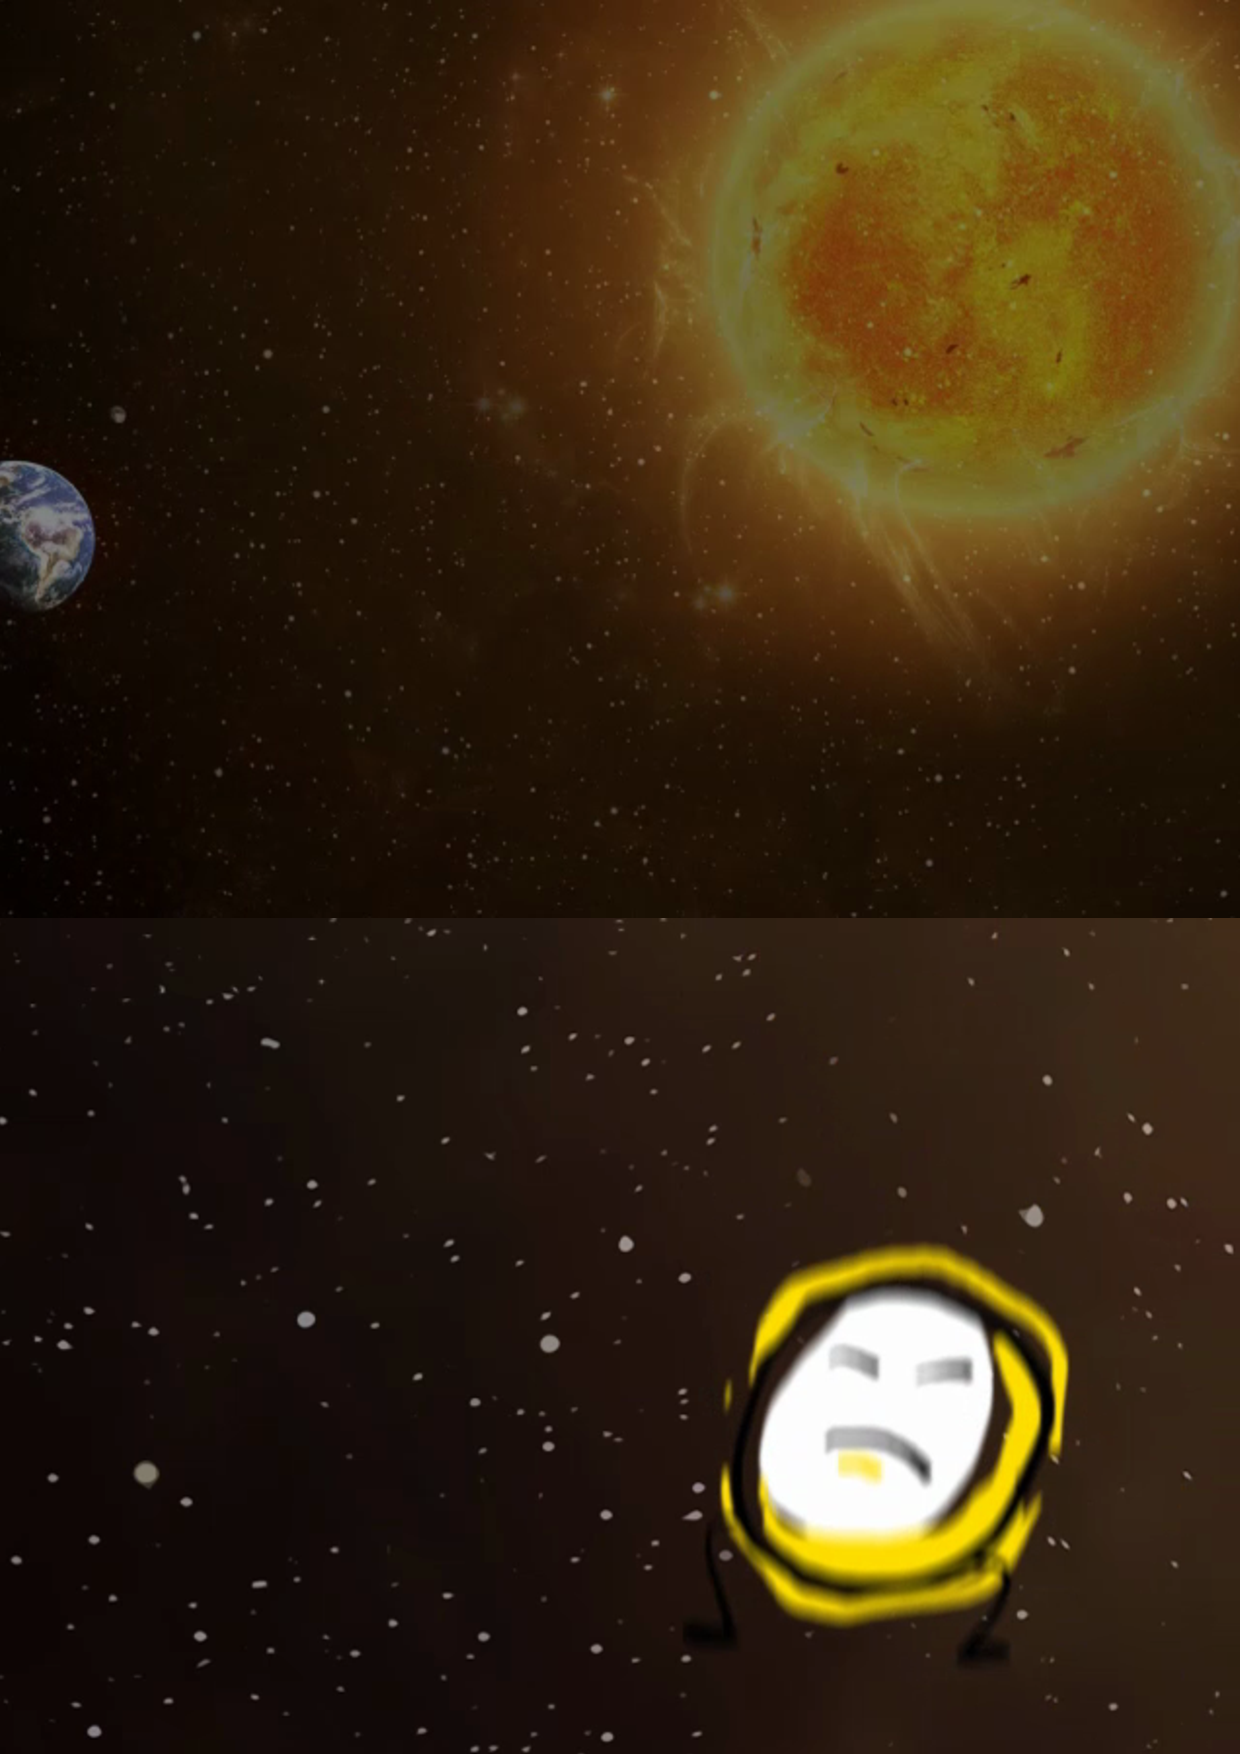
\includegraphics[width=\paperwidth]{frontpage.pdf}}; % Background image
\draw[anchor=north] (midpoint) node [fill=ocre!30!white,fill opacity=1.0,text opacity=1,inner sep=1cm]{\Huge\centering\bfseries\sffamily\parbox[c][][t]{\paperwidth}{\centering EMDO Energy Manager User Manual\\[15pt] % Book title
{\Large Installation, Configuration, Basic Programming, Reference Applications}\\[20pt] % Subtitle
{\huge EMDO can do}}}; % Author name
\end{tikzpicture}};
\end{tikzpicture}
\vfill
\endgroup


%----------------------------------------------------------------------------------------
%	COPYRIGHT PAGE
%----------------------------------------------------------------------------------------

%\newpage
%~\vfill
%\thispagestyle{empty}

%\noindent Copyright \copyright\ 2013 John Smith\\ % Copyright notice

%\noindent \textsc{Published by Publisher}\\ % Publisher

%\noindent \textsc{book-website.com}\\ % URL

%\noindent Licensed under the Creative Commons Attribution-NonCommercial 3.0 Unported License (the ``License''). You may not use this file except in compliance with the License. You may obtain a copy of the License at \url{http://creativecommons.org/licenses/by-nc/3.0}. Unless required by applicable law or agreed to in writing, software distributed under the License is distributed on an \textsc{``as is'' basis, without warranties or conditions of any kind}, either express or implied. See the License for the specific language governing permissions and limitations under the License.\\ % License information

%\noindent \textit{First printing, March 2013} % Printing/edition date

%----------------------------------------------------------------------------------------
%	TABLE OF CONTENTS
%----------------------------------------------------------------------------------------

\chapterimage{photons.png} % Table of contents heading image

%\chapterimage{chapter_head_1.pdf} % Table of contents heading image

\pagestyle{empty} % No headers

 \tableofcontents % Print the table of contents itself

\cleardoublepage % Forces the first chapter to start on an odd page so it's on the right

\pagestyle{fancy} % Print headers again

%----------------------------------------------------------------------------------------
%	PART
%----------------------------------------------------------------------------------------

\part{Parte Uno}

%----------------------------------------------------------------------------------------
%	CHAPTER 1
%----------------------------------------------------------------------------------------

\chapterimage{grid.png} % Chapter heading image

\chapter{Installation}
\section{EMDO101/102/103/104}
\subsection{Features}
The EMDO device is a versatile tool which allows the connection of components such as inverters, chargers, home automation, heat pumps and heaters at your home. It is a versatile piece of electronics that glues everything in the energy infrastructure together.
The EMDO has interfaces already built into the device to facilitate the variety of interconnections with external equipment. The following table lists the interfaces available on the EMDO range of devices:

%include header formatting
%include ticks and cross instead of \Checkmark/NO
%include captions
%\bgroup
\def\arraystretch{1.3}
\begin{tabular}{@{}l  l l l l@{}} \\\hline
					&	EMDO101	&	EMDO102	&	EMDO103	&	EMD104 	\\\hline
D0 magnet mount  & \Checkmark & - & - & - \\
DIN rail mount  &  & \Checkmark & \Checkmark & \Checkmark \\
RS485					&	\Checkmark (1)	&	\Checkmark (2)	&	\Checkmark (1)		&	\Checkmark (1)		\\
D0 interface\footnote{External D0 reader head available for all DIN rail models.}	&	\Checkmark	&		&			&			\\     
M-Bus interface					&		&		&	\Checkmark		&			\\     
KNX interface					&		&		&			&	\Checkmark		\\      
Relay output driver			&	\Checkmark (1)	&	\Checkmark (2)	&	\Checkmark (2)	&	\Checkmark (2)		\\
S0 optical input 			&	\Checkmark	&		&			&			\\
S0 electrical inputs 		&	\Checkmark (2) &	\Checkmark (2)	&	\Checkmark (2)	&	\Checkmark (2)	\\
S0 electrical outputs	&	\Checkmark (2)	&	\Checkmark (2)	&		\Checkmark (2)	& \Checkmark (2)			\\
Expansion Board connector		&	\Checkmark	&	\Checkmark	&	\Checkmark		&	\Checkmark		\\
Board temperature sensor		&	\Checkmark	&	\Checkmark	&	\Checkmark		&	\Checkmark		\\
Ethernet 				&	\Checkmark	&		\Checkmark	&	\Checkmark		&	\Checkmark		\\
USB for firmware update		&	\Checkmark	&	\Checkmark		&	\Checkmark		&	\Checkmark		\\
USB Power supply			&	\Checkmark	&			&			&			\\
DIN Power supply			&		&	\Checkmark & \Checkmark &	\Checkmark \\
Default reset button		&	\Checkmark	&		\Checkmark	&	\Checkmark		&		\Checkmark	 \\\hline
\end{tabular}
%\egroup

\newpage
\section{Pin Diagrams}

%TODO: DANI - include schematic applicable to EMOD10x devices with pin layout, or clear picture

%TODO: Add table of pins for the EMDO10x devices 

%TODO: Single out interfaces which require specific mention
%e.g RS485, mbus, Relay Output Driver, Optical/Electrical ports, board temperature sensor, firmware upgrade

\subsection{EMDO101}
EMDO101 classic is directly assembled on a utility meter on the D0 Interface (IEC-62056-21). Refer to page \ref{EMDO101_Application} for Application.

%TODO: Add picture showing direct mount
%Any other pictures relevant to direct mounting
%TODO: Mention pin One is Red in Color
%TODO: Mention connector Push in spring connector
%TODO: Tabulate pin layout
%TODO: Reference Application Chapter.Modify reference according to requirement. Can show page number, section and chapter number if necessary
%TODO: Use Labels to link to Application Chapter Sections
%TODO: Add description of Pins
\begin{table}[h!]
\caption{EMDO101 device pins}
\label{tbl:EMDO101_pins}
\begin{tabular}{@{}l l p{10cm} @{}}\\\hline
Pin & 	Function 		& Description		\\\hline
1 	&	S0 IN 1 +		& \multirow{4}{10cm}{S0 input with galvanic isolation, see page \pageref{fig:s0_input_application} for details.\newline This port can be used as gpio input or S0 signal counter from an energy meter.\newline 
\textbf{Wrong external wiring might damage devices.}}	\\
2 	&	S0 IN 1 -		& 					\\
3 	&	S0 IN 2 +		&  					\\
4 	&	S0 IN 2 -		& 					\\\hline
5 	&	S0 OUT 1 +		& \multirow{4}{10cm}{S0 output with galvanic isolation, see page \pageref{fig:s0_output_application} for details.\newline This port can be used as gpio output or S0 output generator for an energy meter.\newline 
\textbf{Wrong external wiring might damage devices.}}	\\	
6 	&	S0 OUT 1 -		& 					\\
7 	&	S0 OUT 2 +		& 					\\
8 	&	S0 OUT 2 -		& 					\\\hline
9 	&	GND				& \multirow{2}{10cm}{external power supply up to 200mA} \\
10 	&	5V Out		 	& 					\\\hline
11 	&	RS485 A			& \multirow{2}{10cm}{RS485 transceiver, see page \pageref{fig:rs485_application} for details.}	\\
12 	&	RS485 B			&					\\\hline
13 	&	Relay OUT		& Relay driver output, see page \pageref{fig:relay_application} for details.				\\\hline
\end{tabular}
\end{table}

\begin{center}
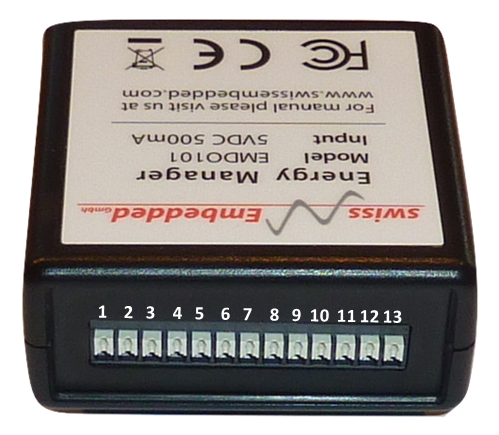
\includegraphics[width=6cm]{P1020554_burnedv1.png}
\end{center}

\begin{comment}
Features now covered in the introduction section
One RS485
one relay output driver
one s0 optical input 
two s0 electrical inputs
two s0 electrical outputs
board temperature sensor
Ethernet 
usb for firmware update
USB Power supply
default reset button
\end{comment}

\newpage
\subsection{EMDO102}
EMDO102 is mounted on a DIN Rail and can be connected with an optional external D0 reader head (IEC-62056-21). Refer to page \ref{EMDO102_DIN_Appplication} for Application.


\begin{table}[h!]
\caption{EMDO102 device pins}
\label{tbl:EMDO102_pins}
\begin{tabular}{@{}l l l @{}}\\\hline
% This is front view, bottom left
Pin & 	Function 		& Description		\\\hline
1 	&	24V IN (or 12V)	& \multirow{2}{10cm}{}	\\
2 	&	GND				& 					\\\hline
3 	&	GND				& \multirow{2}{10cm}{internal fuse protected, approx. 1.4A}					\\
4 	&	24V Out			& \\\hline
5 	&	Relay Out 1		& \multirow{2}{10cm}{Relay driver output, see page \pageref{fig:relay_application} for details.}					\\	
6 	&	Relay Out 2		& 					\\\hline
7 	&	GND (1Wire)		& \multirow{2}{10cm}{1-Wire transceiver, see page \pageref{fig:1wire_application} for details.}					\\
8 	&	1 Wire			& 					\\\hline
\\hline\\hline
% This is front view, top right (numbering from right to left)
Pin & 	Function 		& Description		\\\hline
1 S0 In 1 +
2 S0 In 1 -
3 S0 In 2 +
4 S0 In 2 -
5 	&	5V Out		 	& external power supply up to 0.8A (shared with other port)	\\\hline
6 GND
7 RS485 A2
8 RS485 B2
\\hline\\hline
% This is front view, top left (numbering from right to left)
Pin & 	Function 		& Description		\\\hline
1 S0 Out 1 +
2 S0 Out 1 -
3 S0 Out 2 +
4 S0 Out 2 -
5 	&	5V Out		 	& external power supply up to 0.8A (shared with other port)	\\\hline
6 	&	GND				& \multirow{2}{10cm}{}					\\
7 	&	RS485 A			& \multirow{2}{10cm}{RS485 transceiver, see page \pageref{fig:rs485_application} for details.}					\\
8 	&	RS485 B			&					\\\hline
\end{tabular}
\end{table}

%TOD: pin layout for EMDO102 if necessary
%\begin{center}
%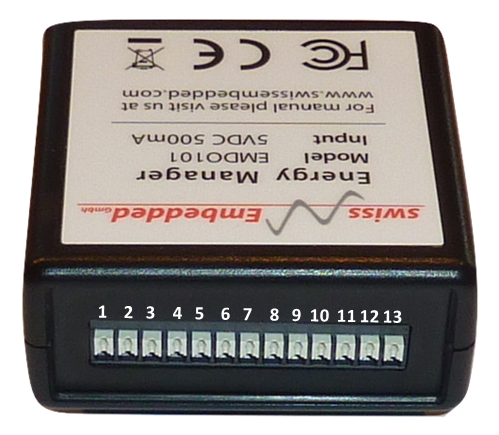
\includegraphics[width=6cm]{P1020554_burnedv1.png}
%\end{center}


%TODO: Add picture showing DIN rail mounting and DO interconnection

\begin{comment}
two rs485
two relay output drivers
two s0 electrical inputs
two s0 electrical outputs
board temperature sensor
1 wire
Ethernet 
usb for firmware update
default reset button
Requires 24V DIN rail power supply
picture emdo102

\end{comment}
\begin{center}
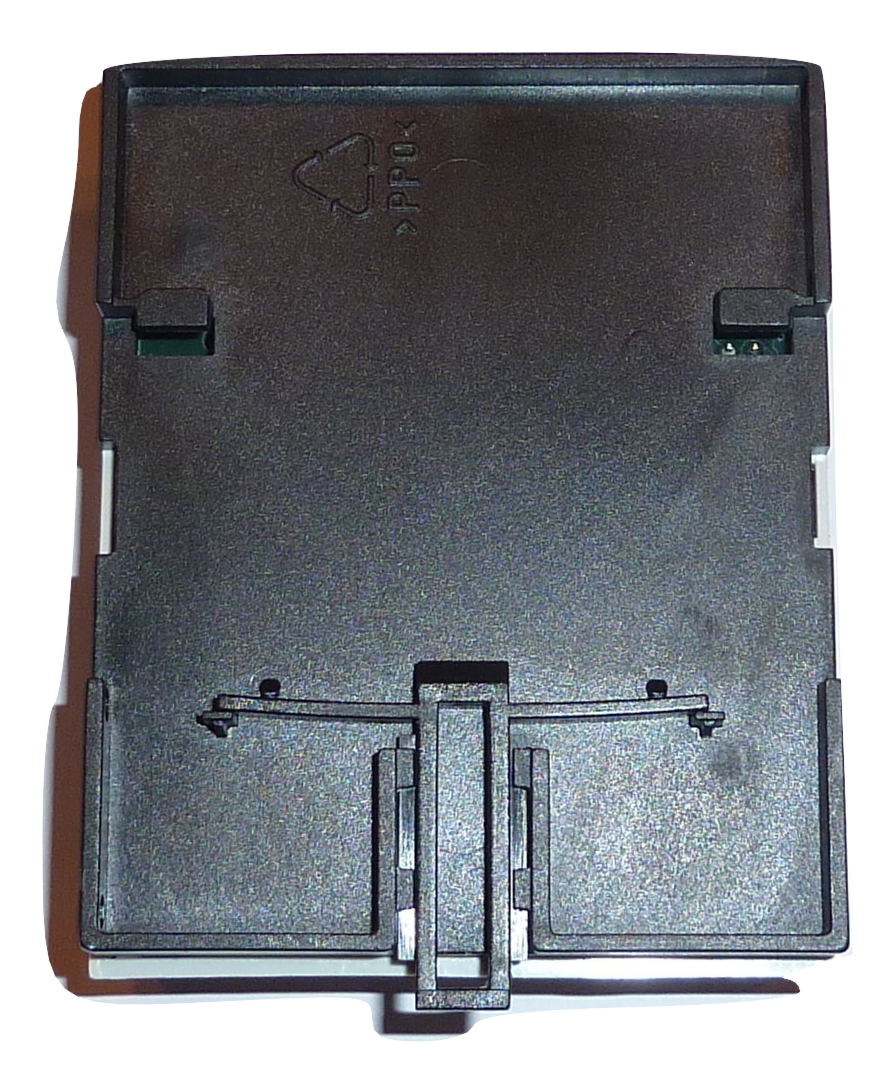
\includegraphics[width=6cm]{P1020571_burned.png}
\end{center}
\begin{center}
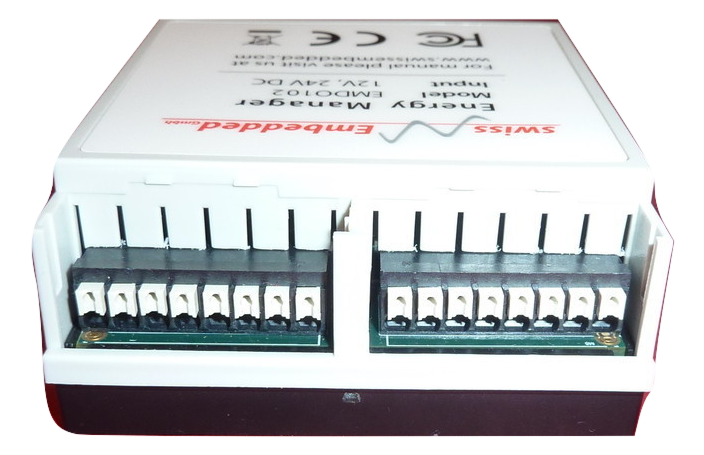
\includegraphics[width=6cm]{P1020575_burned.png}
\end{center}
\begin{center}
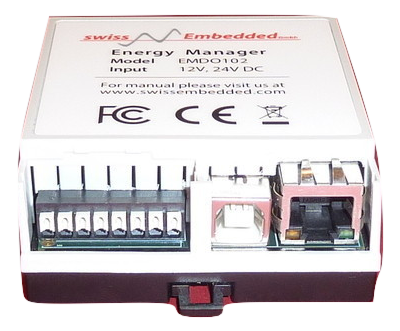
\includegraphics[width=6cm]{P1020578_burned.png}
\end{center}
\begin{center}
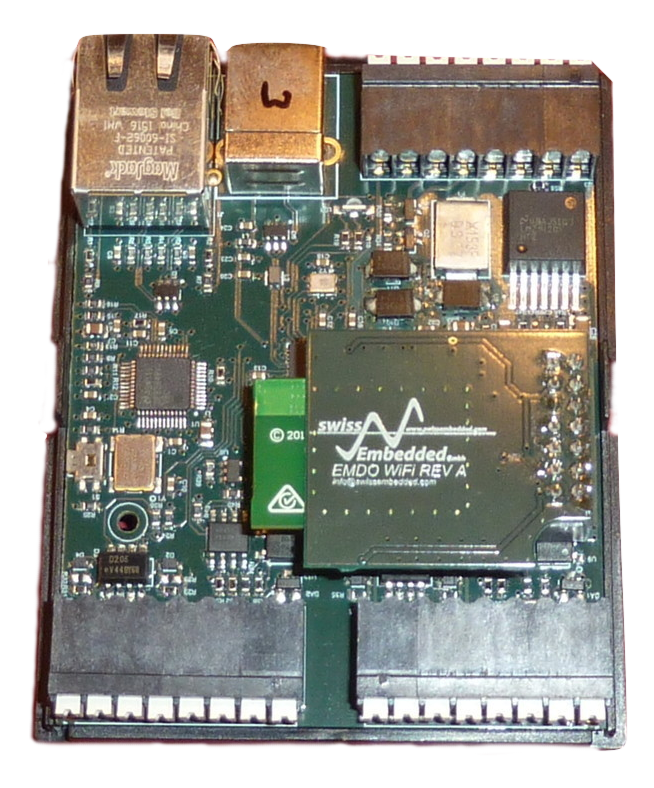
\includegraphics[width=6cm]{P1020567_burned.png}
\end{center}


\newpage
\subsection{EMDO103}
EMDO103 is connected to the meter over the MBUS interface.

\begin{table}
\caption{EMDO103 device pins}
\label{}
\begin{tabular}{@{}l l l @{}}\\\hline
Pin & Function & Description \\\hline
1 & S0 IN 1 + & \\
2 & S0 IN 1 - & \\
3 & S0 IN 2 + & \\
4 & S0 IN 2 - & \\
5 & 5V Out & \multirow{2}{10cm}{approx 0.9A in total} \\
6 & GND & \\
7 & MBUS A & \multirow{2}{10cm}{requires external power supply over bus} \\
8 & MBUS B &  \\\hline
\end{tabular}
\end{table}
%TODO: add picture of emdo103

\subsection*{EMDO104}
EMDO104 is connected to the meter over KNX bus.

%TODO: picture emdo104 if necessary
\begin{tabular}{@{}l l l @{}}\\\hline
Pin & Function & Description \\\hline
1 & S0 IN 1 + & \\
2 & S0 IN 1 - & \\
3 & S0 IN 2 + & \\
4 & S0 IN 2 - & \\
5 & 5V Out (approx 0.9A in total) & \\
6  & GND & \\
7  & KNX A (requires external power supply over bus) & \\
8  & KNX B (requires external power supply over bus) & \\\hline
\end{tabular}


\begin{center}
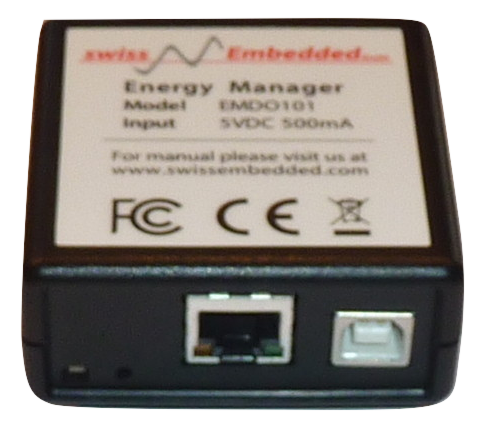
\includegraphics[width=6cm]{P1020553_burned.png}
\end{center}

\begin{center}
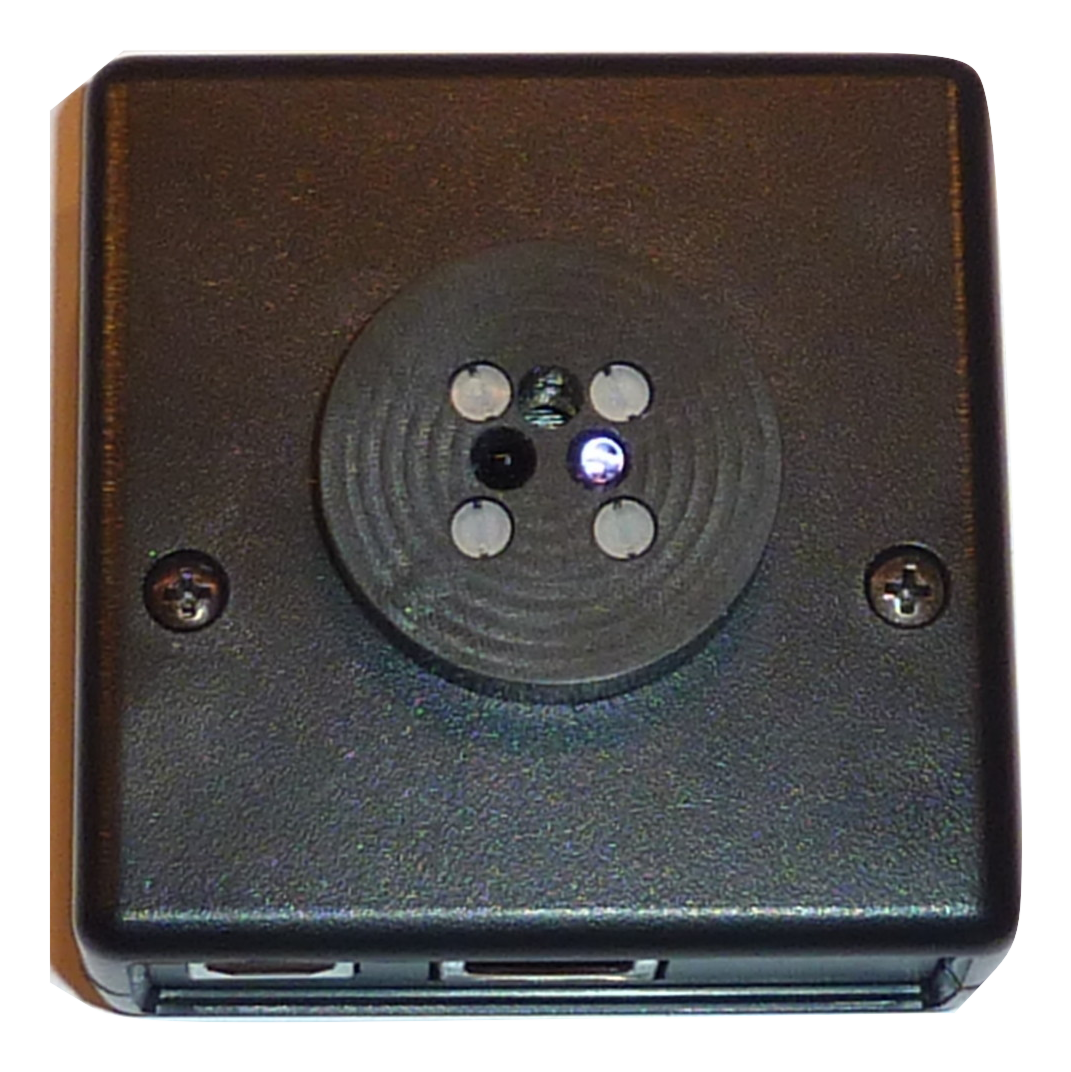
\includegraphics[width=6cm]{P1020569_burned.png}
\end{center}

\subsection*{Expansion boards}
Expansion board is available for the EMDO devices to provide the following interfaces;

\begin{itemize}
\item LoRaWAN
\item WMBUS
\item Enocean
\item Zigbee
\item WiFi
\end{itemize}

%TODO: picture of expansion boards

%Install / deinstall Expansion Board, disconnect power, open EMDO enclosure with two black skews or remove cover
%picture emdo classic skews to open
%picture din rail enclosure open
%put expansion board on header
%for radio modules it is important that electromagnetic radiation is not obscured by walls, metal enclosures,... this greatly disgrades performance.


%----------------------------------------------------------------------------------------
%	CHAPTER 2
%----------------------------------------------------------------------------------------
\chapterimage{hairdryer.png} % Chapter heading image
\chapter{Webinterface}

EMDO runs with dhcp server, however if no dhcp server is present, fixed ip can be used.
if settings are bad and emdo can't be connected anymore with fixed ip, there is a reset button to factory default on the emdo

add pictures from web folderdescribe all pictures, except credits, will go into its own chapter
pictures must be cut on bottom and top that can be done in latex too. pls make pictures again before final manual, we will still change one or the other mask slightly. e.g. tab menu has changed (temp removed).you might take some text from welcome tab.

contact tab: there is support page in case of trouble

network tab (top down): enable dhcp client, set network static settings, ntp server ip or dn , mqtt ip or domain name, remote syslog (rsyslog) server ip or domain name, configure logging, configure remote shell (rsh) should be disabled by default, config tcp to d0 gateway, config tcp to rs485 gateway, auth password.
All data loggin is based on ntp time, thus this is very important.

firmware update tab: System log gives details about system. describe procedure for firmware update from file. Prior to update, make sure data from emdo is copied with get data snapshot. then choose firmware file, there are two files one for program memory on the cpu and second for filesystem. This order should be maintained for firmware updates. 

D0, RS485, S0 Input, S0 Output tab: describe the settings. D0 is for the IEC interface. These settings can also be set from basic interpreter. 

Editor tab: this is the main tab for writing and running a program.  Pls play around with the editor and  describe the buttons. Time is from ntp server, it is not running info is shown. white area with numbers for the source code, blue background area is for print output, variable area to show variable values, buttons to run stop, restart, slow step, upload download the basic interpreter code. it is also possible to upload libraries.
% FIXME add tabs for mbus and knx when available

graphs tab: all data are saved on 32mb flash that is build into the emdo. logger library write data to flash and it is visualized as plots. live data are shown as donuts with text. these data can be configured.

JSON stuff read and write variables
-----------------------------
\chapterimage{panel.png} % Chapter heading image
\chapter{Configuration}


-----------------------------
\chapterimage{cooking.png} % Chapter heading image

\chapter{Application}

%Example referencing
%TODO: Modify reference according to requirement. Can show page number, section and chapter number if necessary
\section*{EMDO101}
\label{EMDO101_Application}
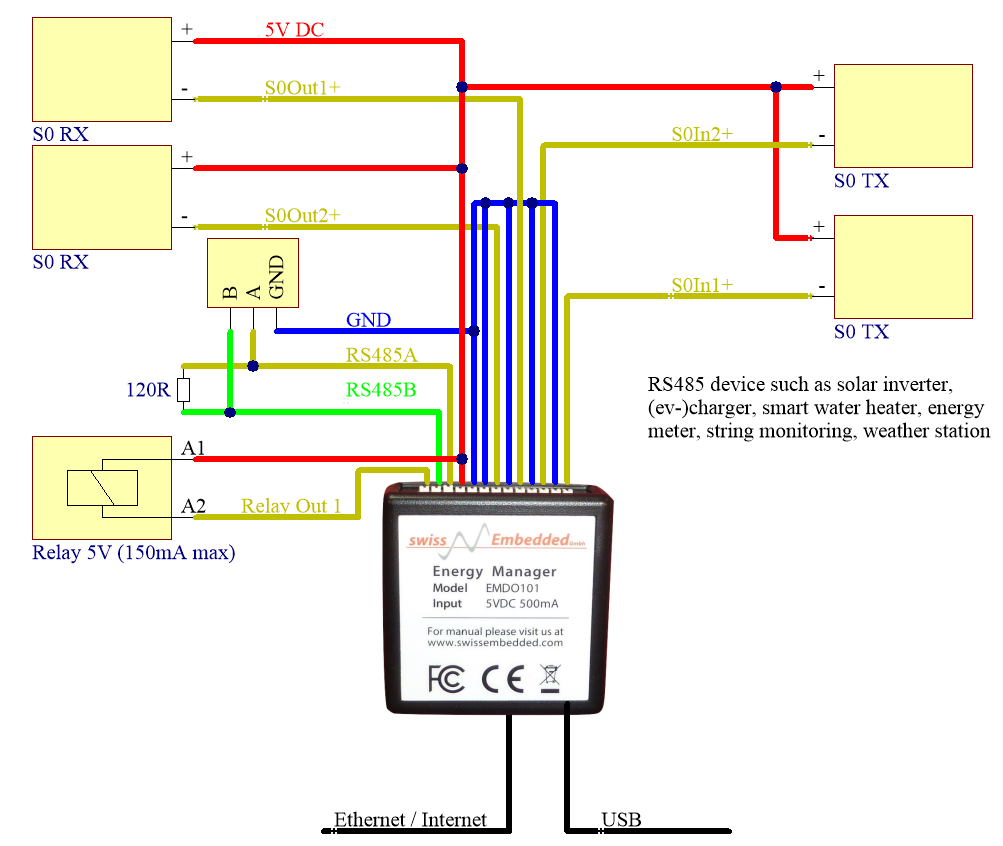
\includegraphics[width=12cm]{application_classic.png}\newline
\section*{EMDO102}
\label{EMDO102_DIN_Appplication}


Temperature sensor based on DS18S20 chip. Example shows parasitic power of the 1-wire chip. 5V power is also available on the connector on the top row.
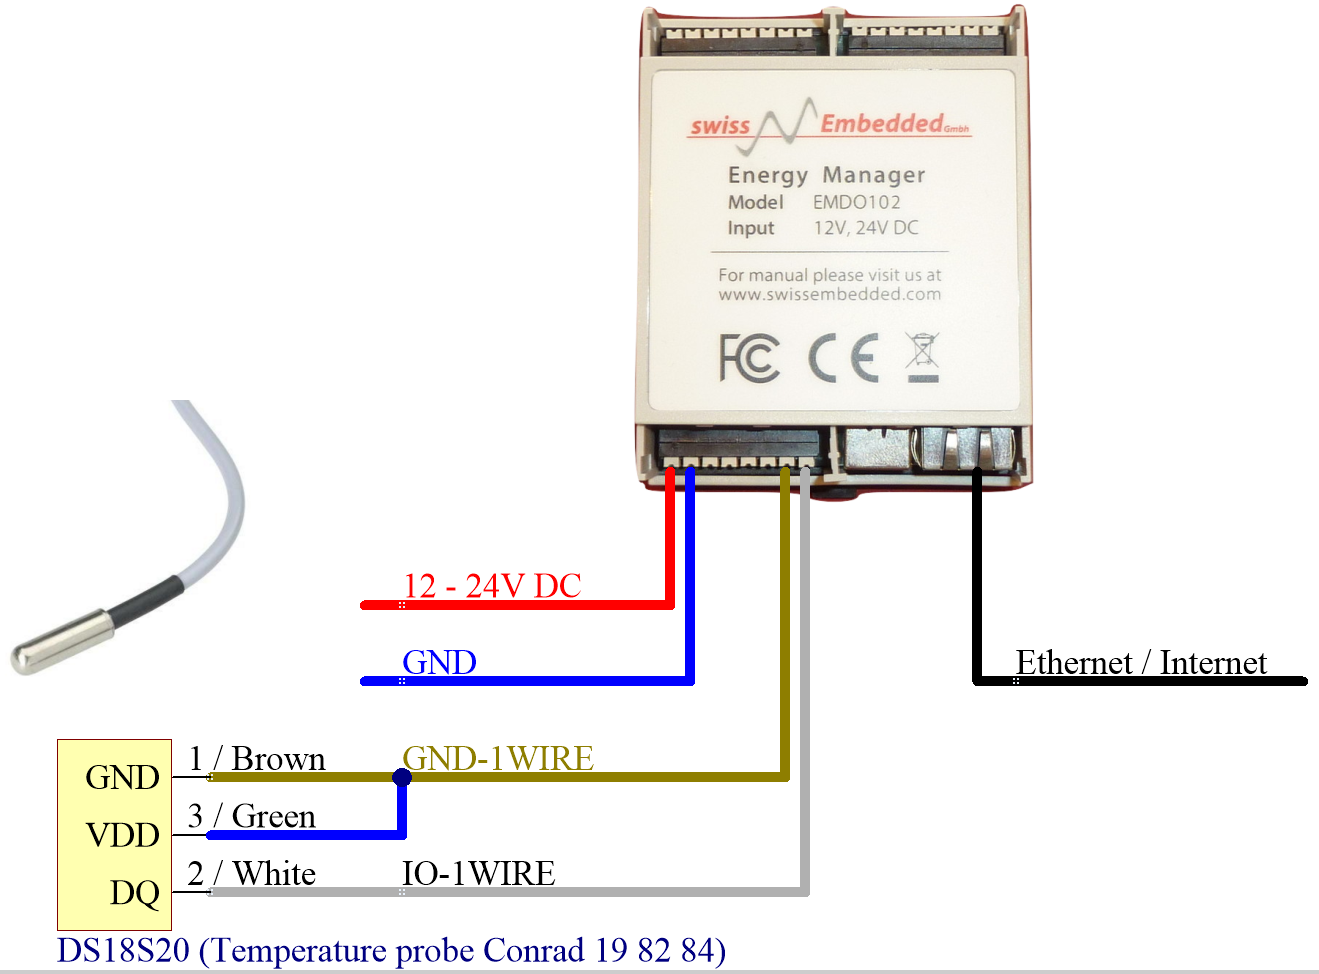
\includegraphics[width=12cm]{application_1-wire-temperature.png}\newline
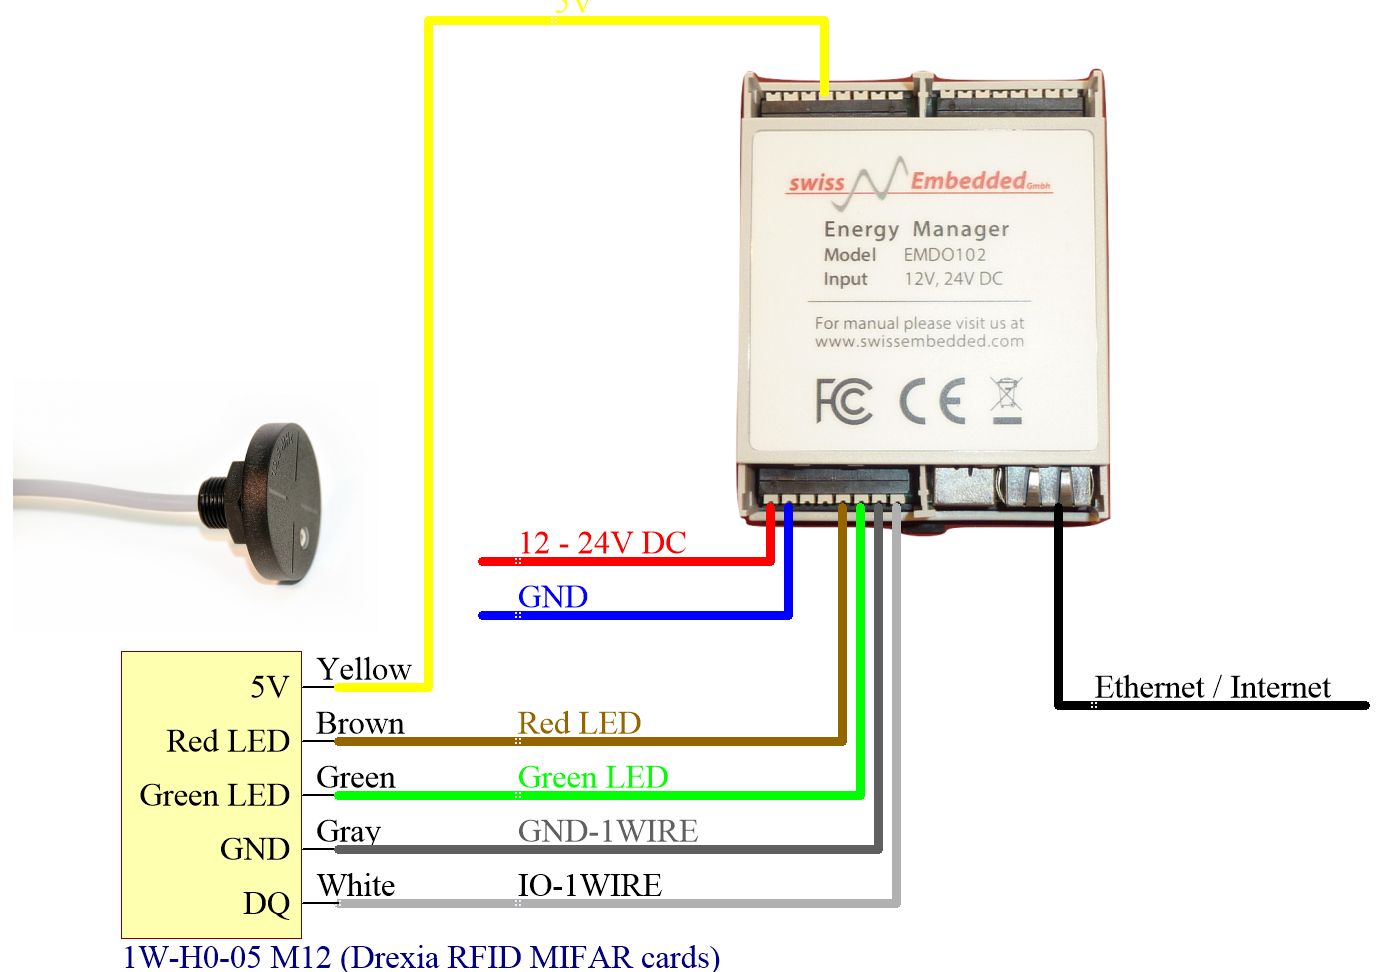
\includegraphics[width=12cm]{application_1-wire-rfid.png}\newline
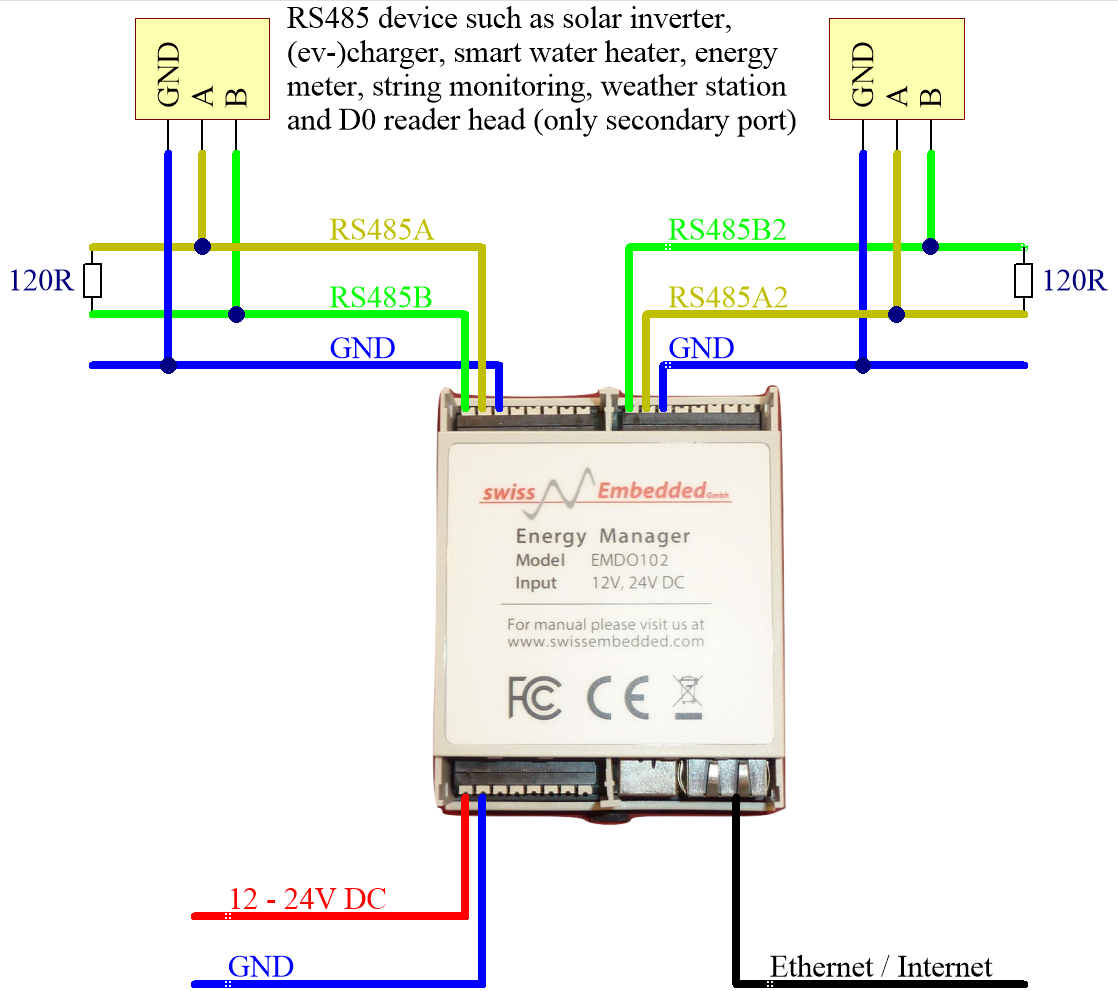
\includegraphics[width=12cm]{application-rs485.png}\newline
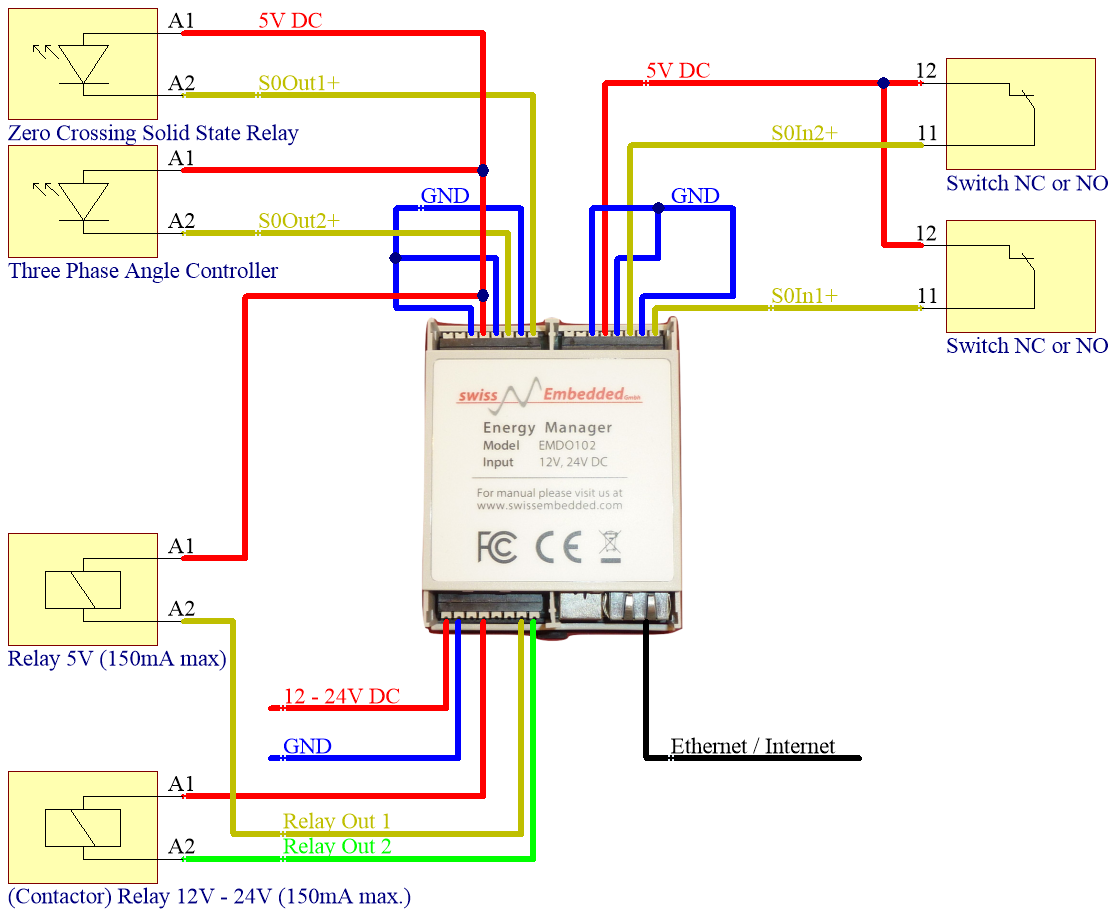
\includegraphics[width=12cm]{application_relay.png}\newline
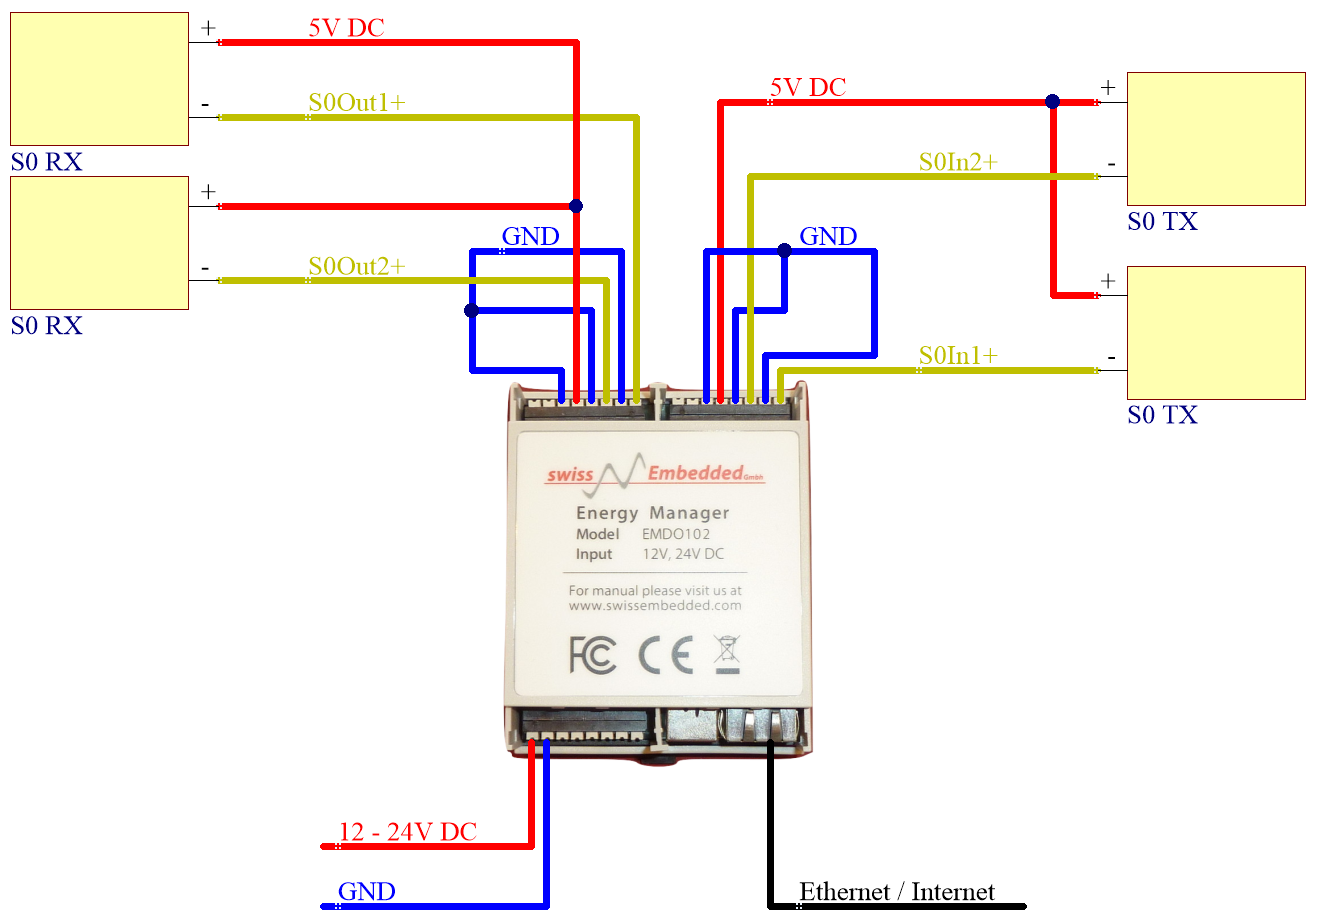
\includegraphics[width=12cm]{application_s0io.png}\newline

\chapter{Basic Interpreter}

reference to mmbasic
table with commands
pls make sure all of these are convered.most should be covered already in the word document. all otheres I can quickly write up for you, once it is in table format. to describe some operator we can take text from mmbasic manual

Square brackets indicate that the parameter or characters are optional.
\begin{table}[]
\centering
\caption{Commands}
\label{Commands}
\begin{tabular}{|p{4cm}|p{10cm}|}
\hline
\textbf{Basic Interpreter} & \textbf{Description}                                                   \\ \hline
\\ \hline
\end{tabular}
\end{table}

\newpage
\begin{center}
\begin{longtable}{l}
\caption{Commands} \label{Commands}\\

\hline
\textbf{Basic Interpreter} \\ 
\hline 
\endfirsthead

\textbf{LIBRARY LOAD} \$file\newline
\textbf{LIBRARY UNLOAD} \$file
\\ Will load a library file ('file\$') into general memory. Any user defined
commands and subroutines in the file will then become available to the
running program.\newline 
A library file is like any other MMBasic program, with the exception
that any programming code outside the user defined commands and
subroutines in the file will be ignored. The library is not visible to the
user (it is not listed by the LIST command) so it should be tested and
debugged as a normal basic program first. Normally a library file has
the extension ".BLIB" and that extension will be automatically added if
the file name ('\$file') does not include the extension.\newline
Libraries can be loaded and unloaded in any order. Libraries can be
loaded from within other libraries and nested to an unlimited extent.
Any library file can be unloaded from memory and the memory returned
to the general pool by using the LIBRARY UNLOAD command.\newline
Library files must not be unloaded from within a library that is currently
being used by the program (the results are undefined but it may crash
MMBasic and cause your hair to go prematurely grey).\newline
This command can be used to load specialised libraries to extend the
functionality of MMBasic. Examples include device drivers, libraries
that provide bit manipulation and libraries of specialised mathematical
functions. The library file is only loaded on the first load command
encountered so it is acceptable to put the same load command into every
part of the program or every subroutine that may need the library.\newline
Another use of the LIBRARY command is to extend the amount of
memory available to a program by only loading sections of code as
needed and then unloading them when their task is finished so that
another function can be loaded.\newline
To prevent fragmentation of memory, functions that use a lot of memory
(like arrays) should be declared first before any
libraries are loaded and then unloaded.bla
\\ \hline
\textbf{LIBRARY LOAD} \$file\newline
\textbf{LIBRARY UNLOAD} \$file
\\ Will load a library file ('file\$') into general memory. Any user defined
commands and subroutines in the file will then become available to the
running program.\newline 
A library file is like any other MMBasic program, with the exception
that any programming code outside the user defined commands and
subroutines in the file will be ignored. The library is not visible to the
user (it is not listed by the LIST command) so it should be tested and
debugged as a normal basic program first. Normally a library file has
the extension ".BLIB" and that extension will be automatically added if
the file name ('\$file') does not include the extension.\newline
Libraries can be loaded and unloaded in any order. Libraries can be
loaded from within other libraries and nested to an unlimited extent.
Any library file can be unloaded from memory and the memory returned
to the general pool by using the LIBRARY UNLOAD command.\newline
Library files must not be unloaded from within a library that is currently
being used by the program (the results are undefined but it may crash
MMBasic and cause your hair to go prematurely grey).\newline
This command can be used to load specialised libraries to extend the
functionality of MMBasic. Examples include device drivers, libraries
that provide bit manipulation and libraries of specialised mathematical
functions. The library file is only loaded on the first load command
encountered so it is acceptable to put the same load command into every
part of the program or every subroutine that may need the library.\newline
Another use of the LIBRARY command is to extend the amount of
memory available to a program by only loading sections of code as
needed and then unloading them when their task is finished so that
another function can be loaded.\newline
To prevent fragmentation of memory, functions that use a lot of memory
(like arrays) should be declared first before any
libraries are loaded and then unloaded.bla
\\ \hline 
\end{longtable}
\end{center}

\begin{table}[]
\centering
\caption{Basic Instructions for Program Control}
\label{Basic_Instructions_for_Program_Control}
\begin{tabular}{|p{4cm}|p{10cm}|}
\hline
\\ \hline
\textbf{CHAIN} file\$ 
& Clear the current program from memory, load the new program ('file\$')
into memory and run it starting with the first line.\newline
Unlike the \textbf{RUN} command this command retains the current state of the
program (ie, the value of variables, open files, open handles, etc). Cron, Timer, SEMP, MSG will be stay active, it is recommended to \textbf{DETACH} all handlers prior to \textbf{CHAIN} and reattach after it.\newline
One program can \textbf{CHAIN} to another which can then chain to another (or
back to the original) an unlimited number of times. As long as a
program can be broken down into modules this command allows
programs of almost unlimited size to be run, even with limited memory.\newline
Communication between the modules can be accomplished by assigning
values to one or more variables which then can be examined by the new
chained program.
Note that another way of squeezing a large program into limited memory
is to use the \textbf{LIBRARY} command.
\\ \hline
\textbf{LIBRARY LOAD} \$file\newline
\textbf{LIBRARY UNLOAD} \$file
& Will load a library file ('file\$') into general memory. Any user defined
commands and subroutines in the file will then become available to the
running program.\newline 
A library file is like any other MMBasic program, with the exception
that any programming code outside the user defined commands and
subroutines in the file will be ignored. The library is not visible to the
user (it is not listed by the LIST command) so it should be tested and
debugged as a normal basic program first. Normally a library file has
the extension ".BLIB" and that extension will be automatically added if
the file name ('\$file') does not include the extension.\newline
Libraries can be loaded and unloaded in any order. Libraries can be
loaded from within other libraries and nested to an unlimited extent.
Any library file can be unloaded from memory and the memory returned
to the general pool by using the LIBRARY UNLOAD command.\newline
Library files must not be unloaded from within a library that is currently
being used by the program (the results are undefined but it may crash
MMBasic and cause your hair to go prematurely grey).\newline
This command can be used to load specialised libraries to extend the
functionality of MMBasic. Examples include device drivers, libraries
that provide bit manipulation and libraries of specialised mathematical
functions. The library file is only loaded on the first load command
encountered so it is acceptable to put the same load command into every
part of the program or every subroutine that may need the library.\newline
Another use of the LIBRARY command is to extend the amount of
memory available to a program by only loading sections of code as
needed and then unloading them when their task is finished so that
another function can be loaded.\newline
To prevent fragmentation of memory, functions that use a lot of memory
(like arrays) should be declared first before any
libraries are loaded and then unloaded.
\\ \hline
\textbf{LIST}\newline
\textbf{LIST} line\newline
\textbf{LIST} -lastline\newline
\textbf{LIST} firstline -\newline
\textbf{LIST} firstline - lastline\newline
& Lists all lines in a program line or a range of lines.
If –lastline is used it will start with the first line in the program. If
startline- is used it will list to the end of the program.
\\ \hline
\textbf(PAUSE)( delay ) & Halt execution of the running program for ‘delay’ mS.
The maximum delay is 2147483647 mS (about 24 days).
\\ \hline
\textbf{REM} string\newline 
\textbf{'} string
& \textbf{REM} allows remarks to be included in a program.
Note the Microsoft style use of the single quotation mark to denote
remarks is also supported and is preferred for better readability of the code.
\\ \hline
\textbf{RUN} [line] [file\$] & Executes the program in memory. If a line number is supplied then
execution will begin at that line, otherwise it will start at the beginning
of the program. Or, if a file name (file\$) is supplied, the current program
will be erased and that program will be loaded from the current drive and
executed. This enables one program to load and run another.\newline
Example: \textbf{RUN} “TEST.BAS”\newline
If an extension is not specified “.BAS” will be added to the file name.
\\ \hline
\end{tabular}
\end{table}

\begin{table}[]
\centering
\caption{Basic Instructions for System and Memory}
\label{Basic_Instructions_for_System_and_Memory}
\begin{tabular}{|p{4cm}|p{10cm}|}
\hline
\textbf{Basic Interpreter} & \textbf{Description}                                                   \\ \hline
\textbf{CLEAR} & Delete all variables and recover the memory used by them. See \textbf{ERASE} for deleting specific array variables.
\\ \hline
\textbf{ERASE} variable
[,variable]...
&
Deletes arrayed variables and frees up the memory. \newline
Use \textbf{CLEAR} to delete all variables including all arrayed variables.
\\ \hline 
\textbf{ERROR} [errormsg\$] & Forces an error and terminates the program. This is normally used in
debugging or to trap events that should not occur.
\\ \hline
\textbf{MEMORY} & List the amount of memory currently in use. For example: \newline
 \textit{\newline 1kB (1\%) Program (9 lines) \newline 1kB (0\%) 5 Variables \newline 0kB (0\%) General \newline 98kB (99\%) Free} \newline \newline
Program memory is cleared by the NEW command. Variable and the general memory spaces are cleared by many commands (eg, \textbf{NEW}, \textbf{RUN}, \textbf{LOAD}, etc) as well as the specific commands \textbf{CLEAR} and \textbf{ERASE}. General memory is used by streams, file I/O buffers, etc.   
\\ \hline
\textbf{PEEK}(VAR var, +-offset)
& Will return a byte within MMBASIC variable memory space.\newline
You can access the memory allocated to a variable by using the
variable's name ('var') preceded by the keyword VAR. This can be used
to access the individual bytes of a numeric variable or a large segment of
RAM allocated to an array (the first element of an array (eg, nbr(0)) is
the start of RAM allocated to the whole array). 'offset' is the offset in the memory space. This depends on the processor architecture and might be incompatible to future EMDO designs. For this reason, We recommend to use the more versatile \textbf{Conv} command for any type of data conversions.
\\ \hline
\end{tabular}
\end{table}

\begin{table}[]
\centering
\caption{Basic Instructions for System (Option)}
\label{Basic_Instructions_for_System_Option}
\begin{tabular}{|p{4cm}|p{10cm}|}
\hline
\textbf{Basic Interpreter} & \textbf{Description}                                                   \\ \hline
\textbf{OPTION BASE} 0\newline
\textbf{OPTION BASE} 1
& Set the lowest value for array subscripts to either 0 or 1. The default is
0. This must be used before any arrays are declared.
\\ \hline
\textbf{OPTION ERROR CONTINUE}\newline
\textbf{OPTION ERROR ABORT}
 & Set the treatment for errors in file input/output. The option \textbf{CONTINUE}
will cause MMBasic to ignore file related errors. The program must
check the variable \textbf{MM.ERRNO} to determine if and what error has
occurred.\newline
The option ABORT sets the normal behaviour (ie, stop the program and
print an error message). The default is \textbf{ABORT}.\newline
Note that this option only relates to errors reading from or writing to
NOR flash. It does not affect the handling of syntax and other
program errors.
\\ \hline
\textbf{OPTION PROMPT} string\$ & Sets the command prompt to the contents of ‘string\$’ (which can also be an expression which will be evaluated when the prompt is printed).\newline
For example:\newline
\textbf{OPTION PROMPT} “Ok “\newline
\textbf{OPTION PROMPT} TIME\$ + “: “\newline
\textbf{OPTION PROMPT} CWD\$ + “: “\newline
Maximum length of the prompt string is 48 characters. The prompt is
reset to the default (“> “) on power up but you can automatically set in the first lines of the program.
\\ \hline
\end{tabular}
\end{table}

\begin{table}[]
\centering
\caption{Basic Instructions for Debug}
\label{Basic_Instructions_for_Debug}
\begin{tabular}{|p{4cm}|p{10cm}|}
\hline
\textbf{Basic Interpreter} & \textbf{Description}                                                   \\ \hline
\textbf{SYSLOG} \textit{log-level}, \textit{log} 
& This mechanism allows to collect logs from EMDO devices centrally and analyze the logs. The open source software Logstash and Kibana is used for this.
\\ \hline
\textbf{SYSTEM} \textit{command\$}
& Execute a command in the EMDO operating system's command line interface. \newline
For example:\newline
\textbf{SYSTEM} "stat s0 clear"
\\ \hline
\textbf{TRACE ON}\newline
\textbf{TRON}\newline
\textbf{TRACE OFF}\newline
\textbf{TROFF}\newline
\textbf{TRACE EXTENDED}\newline
\textbf{TRACE LIST}
&  Turns on/off the trace facility. This facility will print the number of each line
(counting from the beginning of the program) in square brackets as the
program is executed. This is useful in debugging programs.\newline
In some situations more verbose output can be activated with \textbf{EXTENDED}.\newline
As logging has an impact on program execution speed, it is sometime better to list the trace log when the program is idle (\textbf{TRACE LIST}) rather than all the time (\textbf{TRACE ON}). 
\\ \hline
\end{tabular}
\end{table}


\begin{table}[]
\centering
\caption{Basic Instructions for Read Only Variables}
\label{Basic_Instructions_for_Read_Only_Variables}
\begin{tabular}{|p{4cm}|p{10cm}|}
\hline
\textbf{Basic Interpreter} & \textbf{Description}                                                   
\\ \hline
\textbf{MM.VER} & The version number of the firmware in the form aa.bbcc where aa is the major version number, bb is the minor version number and cc is the revision number (normally zero but A = 01, B = 02, etc).
\\ \hline
\textbf{MM.FNAME}\$ & The name of the file that will be used as the default for the \textbf{SAVE} command. This is set by \textbf{LOAD}, \textbf{RUN} and \textbf{SAVE}.
\\ \hline
\textbf{MM.CMDLINE}\$ & The command line used with the implied \textbf{RUN} command. See the implied \textbf{RUN} command at the start of the next page for the details.
\\ \hline
\textbf{MM.ERRNO} & Is set to the error number if a statement involving the NOR flash fails or
zero if the operation succeeds. This value is not supported yet.
\\ \hline
\textbf{COPYRIGHT}
& Show MMBASIC copyright.
\\ \hline
\end{tabular}
\end{table}


\begin{table}[]
\centering
\caption{Basic Instructions for IO Open and Close}
\label{Basic_Instructions_for_IO_Open_Close}
\begin{tabular}{|p{4cm}|p{10cm}|}
\hline
\textbf{Basic Interpreter} & \textbf{Description}                                                   \\ \hline
\textbf{OPEN} fname\$ \textbf{FOR} mode
\textbf{AS} [\#]fnbr
& Opens a file for reading or writing.
‘fname’ is the filename with maximal string length (case-sensitive). It can be prefixed with a directory path. For example: "DIR1/DIR2/FILE.EXT". SPIFFS does not support directories. Directories are only emulated. \newline
‘mode’ is \textbf{INPUT}, \textbf{OUTPUT}, \textbf{APPEND} or \textbf{RANDOM}.\newline\newline
\textbf{INPUT} will open the file for reading and throw an error if the file does
not exist. \newline
\textbf{OUTPUT} will open the file for writing and will automatically
overwrite any existing file with the same name.\newline
\textbf{APPEND} will also open the file for writing but it will not overwrite an
existing file; instead any writes will be appended to the end of the file. If
there is no existing file the APPEND mode will act the same as the
\textbf{OUTPUT} mode (i.e. the file is created then opened for writing). \newline
Note:\newline
\textbf{RANDOM} will open the file for both read and write and will allow
random access using the SEEK command. When opened the read/write
pointer is positioned at the end of the file.\newline
‘fnbr’ is the file number (1 to 10). The \# is optional. Up to 10 files can
be open simultaneously. The \textbf{INPUT}, \textbf{LINE INPUT}, \textbf{PRINT}, \textbf{WRITE}
and \textbf{CLOSE} commands as well as the \textbf{EOF}() and \textbf{INPUT\$}() functions all
use ‘fnbr’ to identify the file being operated on.\newline
See also OPTION ERROR and MM.ERRNO for error handling.
\\ \hline
\textbf{CLOSE} [\#]nbr [,[\#]nbr] … &
Close the file(s) previously opened with the file number ‘nbr’.
The \# is optional. Also see the \textbf{OPEN} command.
\\ \hline
\end{tabular}
\end{table}

\begin{table}[]
\centering
\caption{Basic Instructions for IO and File Operation}
\label{Basic_Instructions_for_IO_and_File_Operation}
\begin{tabular}{|p{4cm}|p{10cm}|}
\hline
\textbf{Basic Interpreter} & \textbf{Description}                                                 
\\ \hline
\textbf{INPUT} ["prompt string\$";]
list of variables
& Allows input from the keyboard to a list of variables. The input
command will prompt with a question mark (?).\newline
The input must contain commas to separate each data item if there is
more than one variable.\newline
For example, if the command is:\newline
\textbf{INPUT} a, b, c\newline
And the following is typed on the keyboard: 23, 87, 66\newline
Then a = 23 and b = 87 and c = 66\newline
If the "prompt string\$" is specified it will be printed before the question
mark. If the prompt string is terminated with a comma (,) rather than the
semicolon (;) the question mark will be suppressed.
\\ \hline
\textbf{INPUT}\$(nbr, [\#]fnbr) & Will return a string composed of ‘nbr’ characters read from a file
previously opened for INPUT with the file number ‘fnbr’. This function
will read all characters including carriage return and new line without
translation.\newline
When reading from a serial communications port this will return as
many characters as are waiting in the receive buffer up to ‘nbr’. If there
are no characters waiting it will immediately return with an empty string.\newline
The \# is optional. Also see the\textbf{OPEN} command.
\\ \hline
\textbf{INKEY}\$ & Checks the input of a character.
\\ \hline
\textbf{LINE INPUT} [prompt\$,] string-variable\$\newline
\textbf{LINE INPUT} \#nbr,
string-variable\$
 &  Reads entire line from the keyboard into ‘string-variable\$’. If specified
the ‘prompt\$’ will be printed first. Unlike \textbf{INPUT}, \textbf{LINE INPUT} will
read a whole line, not stopping for comma delimited data items.
A question mark is not printed unless it is part of ‘prompt\$’.
\\ \hline
\textbf{PRINT} expression [[,; ]expression] … etc\newline
\textbf{?} expression [[,; ]expression] … etc
& Outputs text to the browser. Multiple expressions can be used and must be
separated by either a: \newline
\textbf{?} Comma (,) which will output the tab character \newline
\textbf{?} Semicolon (;) which will not output anything (it is just used to separate expressions).\newline
\textbf{?} Nothing or a space which will act the same as a semicolon.\newline
A semicolon (;) at the end of the expression list will suppress the
automatic output of a carriage return/ newline at the end of a print
statement.\newline
When printed, a number is preceded with a space if positive or a minus
(-) if negative but is not followed by a space. Integers (whole numbers)
are printed without a decimal point while fractions are printed with the
decimal point and the significant decimal digits. Large numbers (greater
than six digits) are printed in scientific format.\newline
The function \textbf{FORMAT\$()} can be used to format numbers. The function
\textbf{TAB()} can be used to space to a certain column and the string functions
can be used to justify or otherwise format strings.
\\ \hline
\textbf{PRINT} \#nbr, expression
[[,; ]expression] … etc
& Same as above except that the output is directed to a file previously
opened for \textbf{OUTPUT} or \textbf{APPEND} as ‘nbr’. See the \textbf{OPEN} command.
\\ \hline
\end{tabular}
\end{table}

\begin{table}[]
\centering
\caption{Basic Instructions for SPIFFS File System}
\label{Basic_Instructions_for_SPIFFS_File_System}
\begin{tabular}{|p{4cm}|p{10cm}|}
\hline
\textbf{Basic Interpreter} & \textbf{Description}                                                   
\\ \hline
\textbf{Copy} src\$ To dest\$ & Copy the file named 'src\$' to another file named 'dest\$'.
\\ \hline
\textbf{Dir\$}( \textit{fspec} )\newline
\textit{file-name\$} = \textbf{Dir\$}( )\newline
& Will search the NOR flash for files and return the names of entries found.
\textit{fspec} is a file specification using wildcards the same as used by the
FILES command. E.g., "*.*" will return all entries, "*.TXT" will return
text files.\newline
The function without argument, will return the first entry found. To retrieve subsequent
entries use the function with no arguments. ie, \textbf{DIR\$}. The return of
an empty string indicates that there are no more entries to retrieve.\newline
This example will print all the files in a directory:\newline
\textit{f\$} = \textbf{Dir\$}("*.*")\newline
\textbf{Do While} \textit{f\$} <> ""\newline
\textbf{Print} f\$\newline
\textit{f\$} = \textbf{Dir\$}()\newline
\textbf{Loop}\newline
SPIFFS does not support directories. Leading path alike pattern will force search within a "directory".
\\ \hline
\textbf{Eof}( [\#]nbr ) & Will return true if the file previously opened for INPUT with the file
number ‘nbr’ is positioned at the end of the file.
If used on a file number opened as a serial port this function will return
true if there are no characters waiting in the receive buffer.
The \# is optional. Also see the OPEN, INPUT and LINE INPUT
commands and the \textbf{INPUT\$} function.
\\ \hline
\textbf{FILES} [fspec\$] 
&  Lists files in the current directory of the NOR flash.\newline
Optional use of ‘fspec\$’. Question marks
(?) will match any character and an asterisk (*) will match any number
of characters. If omitted, all files will be listed. For example:\newline
*.* Find all entries\newline
*.TXT Find all entries with an extension of TXT\newline
E*.* Find all entries starting with E\newline
X?X.* Find all three letter file names starting and ending with X
\\ \hline
\textbf{LOC}( [\#]fnbr ) & For a file opened as \textbf{RANDOM} this will return the current position of the read/write pointer in the file. Note that the first byte in a file is
numbered 1. The \# is optional.
\\ \hline
\textbf{LOF}( [\#]fnbr ) & For a file this will return the current length of the file in bytes.
The \# is optional.
\\ \hline
\textbf{KILL} file\$ & Deletes the file specified by ‘file\$’. If there is an extension it must be
specified.\newline
If 'file' is a string constant quote marks around it are optional at the
command prompt but must be specified if the command is used within a
program. Example: \textbf{KILL} “SAMPLE.DAT”
\\ \hline
\textbf{NAME} old\$ AS new\$ 
& Rename a file or a directory from ‘old\$’ to ‘new\$’
Unlike the other commands that work with file names the \textbf{NAME}
command cannot accept a full pathname (with directories).
\\ \hline
\\ \hline
\textbf{SEEK} [\#]fnbr, pos & Will position the read/write pointer in a file that has been opened for RANDOM access to the 'pos' byte.\newline
The first byte in a file is numbered one so \textbf{SEEK} \#5,1 will position the read/write pointer to the start of the file.
\\ \hline
\textbf{POS}() & Returns the current cursor position in the line in characters.
\end{tabular}
\end{table}


\begin{table}[]
\centering
\caption{Basic Instructions for S0 and Relay}
\label{Basic_Instructions_for_S0_relay}
\begin{tabular}{|p{4cm}|p{10cm}|}
\hline
\textbf{Basic Interpreter} & \textbf{Description}                                                   \\ \hline
\textit{pulse-count\%} = \textbf{S0In} ( \textit{port\%} [, \textit{info\$} )\newline
\textit{pulse-count\%} = \textbf{S0In} ( \textit{port\%} [, \textit{reset-counter\%} )
& The S0 and relay outputs are highly configurable to static and dynamic modes. Prior to using a \textit{port\%} it must be configured with \textbf{SYS.SET} for its operation.\newline
Examples:\newline
' TOn, TOff are the minimal on and off period of the pulse in ms. ThHi and ThLo the threshold values of the ADC for high and low signal detection. If the reset flag is set to 1, the current pulse counter is reset.\newline
\textbf{SYS.SET} "s0\_in0", "TOn=30 TOff=30 ThHi=700 ThLo=400 reset=1"\newline
' Read pulse-count from primary S0 input and reset the pulse-count.\newline
\textit{pulse-count\%} = \textbf{S0In}(0,1)\newline       
' Get static state of the first S0 input\newline
\textit{input-state} = \textbf{S0In}(0,'s')\newline
' Get pulse rise time of the first S0 input\newline
\textit{input-state} = \textbf{S0In}(0,'T')\newline
' Get pulse fall time of the first S0 input\newline
\textit{input-state} = \textbf{S0In}(0,'t')\newline
' Get average pulse on time of the first S0 input\newline
\textit{input-state} = \textbf{S0In}(0,'P')\newline
' Get average pulse off time of the first S0 input\newline
\textit{input-state} = \textbf{S0In}(0,'p')\newline
The average pulse times are interesting to calculate average value e.g. for power production or consumption from the counts.
\\ \hline
\textbf{S0Out} \textit{port\%}, \textit{pulse-count\%} [, \textit{blank-period\%}]
& The S0 and relay outputs are highly configurable to several static and dynamic modes. Prior to using a \textit{port\%} it must be configured with \textbf{SYS.SET} for its operation.\newline
Examples:\newline
' set first S0 output to 0 (phototransistor or relay driver conducting)\newline
\textbf{SYS.SET} "s0\_out0", "state=0"\newline
' set second S0 output to 1 (phototransistor or relay driver conducting)\newline
\textbf{SYS.SET} "s0\_out1", "state=1"\newline
' set second S0 output to pulsed mode with TOn and TOff period of 30m.\newline
\textbf{SYS.SET} "s0\_out1", "TOn=30000 TOff=30000 mode=1"\newline
' generate 100 pulses  (\textit{pulse-count\%}) on second S0 output\newline
\textbf{S0Out} 1,100\newline
' generate 2 pulses (\textit{pulse-count\%}) on second S0 output with 1 second \textit{blank-period}. This feature is usefull if the device receiving the pulse measures the time between the pulses to calculate a power value from it.\newline
\textbf{S0Out} 1,2, 1000
\\ \hline
\end{tabular}
\end{table}

The EMDO supports the OASIS Standard MQTT v3.1.1. The standard is freely available from \url{http://mqtt.org}.\newline
MQTT (MQ Telemetry Transport) is a protocol for machine to machine communication. It is a publish/subscribe protocol, extremely simple and lightweight messaging protocol, designed for constrained devices and low-bandwidth, high-latency or unreliable networks. The design principles are to minimise network bandwidth and device resource requirements whilst also attempting to ensure reliability and some degree of assurance of delivery. \newline
These principles also turn out to make the protocol ideal of the emerging “machine-to-machine” (M2M) or “Internet of Things” world of connected devices. With this connectivity, it is extremely important that modern encryption technologies are used as much as possible, otherwise private data quickly become public.\newline
For certificate generation please see subsection \ref{subsection:Certificates}.\newline\newline

\begin{table}[h!]
\centering
\caption{Basic Instructions for MQTT Communication}
\label{Basic_Instructions_for_MQTT_Communication}
\begin{tabular}{|p{4cm}|p{10cm}|}
\hline
\textbf{Basic Interpreter} & \textbf{Description}
\\ \hline
\textit{err\%} = \textbf{MQTTConnect}( \textit{server\$, port\%, id\$, connection-flag\$, user\$, pass\$, willtopic\$, willmessage\$, timeout\%})\newline
\textbf{MQTTConnectTLS}( \textit{server\$, port, id\$, connection-flag\$, caCert\$, cliCert\$, cliKey\$, user\$, pass\$, willtopic\$, willmessage\$, timeout\%})
&
Establish a connection to a MQTT broker. We recommend to use the TLS version of the command if you publish or subscribe private data in the cloud.\newline
\textit{server\$} server IP or domain name, use IPMQTT default from network tab on empty string.\newline
\textit{port} server port, if 0 default TCP port 1883 is used.\newline 
\textit{id\$} this is a unique id for a client, best use EMDO unique id \textbf{SYS.GET}(\textit{"asset","serialID"})\newline
\textit{connection-flag\$} for example "C0", where\newline
    C = Clean session\newline
	R = Will Retain (must be not be set if \textit{willmessage} is empty)\newline
	0 = Will QoS0 (at most once delivery)\newline
	1 = Will QoS1 (at least once delivery)\newline
 	2 = Will QoS2 (exactly once delivery)\newline
\textit{caCert\$} file name of the certification authority signed certificate (TLS only)\newline 
\textit{cliCert\$} file name of the client certificate (TLS only)\newline 
\textit{cliKey\$} file name of the client key (TLS only)\newline 
\textit{user\$} authentification username (empty if unused)\newline 
\textit{pass\$} authentification passwort (empty if unused)\newline 
\textit{willtopic\$} will topic (empty if unused)\newline  
\textit{willmessage\$} will message (empty if unused)\newline 
\textit{timeout\%} communication timeout (in ms, -1 if forever)\newline 
Return value 0 on success or error code with negative sign.
\\ \hline
\textit{err\%} = \textbf{MQTTDisconnect}( \textit{timeout} )
&
Wait for disconnect from MQTT broker within the given \textit{timeout\%}.
Return value 0 on success or error code with negative sign.
\\ \hline
\textit{err\%} = \textbf{MQTTPublish}( \textit{flag\$}, \textit{topic\$}, \textit{payload\$}, \textit{timeout\%} )
&
Publish a message through the MQTT broker within the given \textit{timeout}.
\textit{flag\$} for example "DR0", where\newline
   D = DUP flag (this is a possible redelivery)\newline
   R = Retain flag (message must be stored by broker and delivered to new subscribers)\newline
   0 = QoS0 (at most once delivery)\newline
   1 = QoS1 (at least once delivery)\newline
   2 = QoS2 (exactly once delivery)\newline
Return value 0 on success or error code with negative sign.
\\ \hline
\textit{err\%} = \textbf{MQTTSubscribe}( \textit{qos\$}, \textit{topic\$}, \textit{timeout\%})
&
Subscribe to MQTT broker for \textit{topic\$} filter and maximal QoS level of \textit{qos\$} that the MQTT broker is allowed to deliver messages within the given \textit{timeout\%}.\newline
\textit{qos\$} for example "0", where \newline
   0 = QoS0\newline
   1 = QoS1\newline
   2 = QoS2\newline
Return value 0 on success or error code with negative sign.   
\\ \hline
\textit{err\%} = \textbf{MQTTUnsubscribe}( \textit{topic\$}, \textit{timeout\%})
&
Unsubscribe from MQTT broker topic \textit{topic\$} within the given \textit{timeout\%}.\newline
Return value 0 on success or error code with negative sign.
\\ \hline
\textit{num-of-messages\%} = \textbf{MQTTSubscription}( \textit{flag\$}, \textit{topic\$}, \textit{payload\$} )
& 
Poll a received message from the MQTT message queue. The string variables \textit{flag\$}, \textit{topic\$} and \textit{payload\$} will be overwritten by the message. If the message is longer than the maximal string lenght, it will be truncated.\newline 
Return value is the number of messages retrieved (\textit{num-of-messages\%} is 1 on success).
\\ \hline
\end{tabular}
\end{table}

The D0 interface (IEC62056-2) has several operation modes. Typically the device is used in mode C (active) or mode (U) passive mode. Pls make sure the interface is correctly configured.\\newline
This example configures the interface to passive mode: \newline
\textbf{SYS.SET "d0", "mode=U baud=19200 data=8 stop=1 parity=n echo=0 auto-parity=0 strip-parity=0 autoread=0"}.\newline
If the EMDO is configured as D0 to TCP/IP Gateway, the autoread mode queries a new read cycle automatically on each connection. With this mechanism it is possible to read D0 meter periodically, e.g. via Openhab or FHEM by a simple query script.

\begin{table}[h!]
\centering
\caption{Basic Instructions for D0 Communication}
\label{Basic_Instructions_for_D0_Communication}
\begin{tabular}{|p{4cm}|p{10cm}|}
\hline
\textbf{Basic Interpreter} & \textbf{Description}
\\ \hline
\textit{success\%} = \textbf{D0Start}( \textit{ timeout\%} )\newline
& Start a new D0 active readout cycle within the given \textit{timeout\%} (in ms, -1 if forever). Energy meter must be configured in mode A,B,C and E (see IEC62056-2). Mode U is a passive mode and does not require any active readout cycle start. Energy meter periodically outputs all OBIS codes. Return positive value on success. 
\\ \hline
\textit{success\%} = \textbf{D0End}( \textit{ timeout\%} )\newline
& End currently active D0 readout cycle within the given \textit{timeout\%}. Returns positive value on success.
\\ \hline
\textit{OBIS-code\$} = \textbf{D0ReadLn\$}(\textit{ timeout\%} )\newline
& Return an OBIS code (\textit{OBIS-string\$}) per call within the given \textit{timeout\%}. Return an empty string on end.
\\ \hline
\textit{string\$} = \textbf{D0Read\$}(\textit{ num-of-chars\%} )\newline
& Read a string with length \textit{ num-of-chars\%} from the D0 interface. Return the \textit{string\$}. This call is blocking and should only be used in blocking mode.
\\ \hline

\textit{char-int\%} = \textbf{D0Read}()\newline
& Read a character from the D0 interface and return an ASCII value. This call is blocking and should only be used in passive mode. 
\\ \hline

\textit{num-of-chars-written\%} = \textbf{D0Write}( [\textit{string\$}, \textit{char-int\%}, \textit{char-float}] )\newline
& Write the characters from argument to the D0 interface. This call is blocking until all arguments has been sent.
\\ \hline
\end{tabular}
\end{table}

RS485 is a common communication interface. The EMDO does not have any galvanic isolation on the RS485. So make sure that the connected devices have galvanic isolation (most do). If this is not the case, use a RS485 to Ethernet Gateway and connect the device over Ethernet.\newline
RS485 must have termination resistors on both ends of the twisted pair line. EMDO has a software configurable termination resistor incorporated.\newline
RS485 devices use different settings for baudrate, parity and framing. These settings must be configured for all bus participants.\newline
For example \textbf{SYS.SET "rs485-1", "baud=115200 data=8 stop=1 parity=n"}.\newline

\begin{table}[h!]
\centering
\caption{Basic Instructions for RS485 Communication}
\label{Basic_Instructions_for_RS485_Communication}
\begin{tabular}{|p{4cm}|p{10cm}|}
\hline
\textbf{Basic Interpreter} & \textbf{Description}
\\ \hline
\textit{string\$}=\textbf{RS485Read\$}( \textit{device\%}, \textit{num-of-chars\%},  \textit{timeout\%} )
& Read string of \textit{num-of-chars\%} characters from RS485 on port \textit{device\%} (1=first, top left in mounted enclosure front view), within \textit{timeout\%} ms (in ms, -1 if forever). 
\\ \hline
\textit{string\$} = \textbf{RS485ReadLn\$}( \textit{device\%}, \textit{timeout\%}, \textit{end-of-line-token\$} )
& Read string terminated with token \textit{end-of-line-token\$} from RS485 on port \textit{device\%} (1=first, top left in mounted enclosure front view), within \textit{timeout\%} ms (in ms, -1 if forever).\newline 
Some protocol use a fixed line termination like carriage return, line feed at the end of each message. 
\\ \hline
\textit{char-int\%} = \textbf{RS485Read}( \textit{device\%} )
& Read one character from RS485 port \textit{device\%} and return character (\textit{char-int\%}).
\\ \hline
\textit{num-of-chars-written\%} = \textbf{RS485Write}( \textit{device\%}[, \textit{string\$}, \textit{char-int\%}, \textit{char-float}] )
& Write over RS485 \textit{string\$}, \textit{char-int\%} or \textit{char-float} on port \textit{device\%}. Return \textit{num-of-chars-written\%}.
\\ \hline
\end{tabular}
\end{table}

\begin{table}[h!]
\centering
\caption{Basic Instructions for Network Communication}
\label{Basic_Instructions_for_Network_Communication}
\begin{tabular}{|p{4cm}|p{10cm}|}
\hline
\textbf{Basic Interpreter} & \textbf{Description}
\\ \hline
\textit{socket\%} = \textbf{SocketServer} ( \textit{isTCP\%}, \textit{port\%} )
&
Opens a TCP ( \textit{isTCP\%} = 1 ) or UDP server ( \textit{isTCP\%} = 0 ) socket on port \textit{port\%} on the EMDO. On success, the connection handle (\textit{socket\%}) is returned. Negative value on error.\newline
EMDO uses the following ports 23 (telnet TCP), 80 (HTTP TCP), 514 (rsh, TCP), 2020 (TCP to D0 Gateway), 2021 (TCP to RS485 Gateway), 2023 (TCP to RS485-2 Gateway), 9522 (Speedwire, UDP), 1900 (SSDP UDP). These ports are not available.
\\ \hline
\textit{socket\%} = \textbf{SocketClient}(\textit{isTCP\%}, \textit{server\$}, \textit{port\%})
& Opens a TCP ( \textit{isTCP\%} = 1 ) or UDP client ( \textit{isTCP\%} = 0 ) connection to the remote \textit{server\$} (IP or domain name) on port \textit{port\%}. On success, the connection handle (\textit{socket\%}) is returned. Negative value on error.\newline
\\ \hline
\textit{is-connected\%} = \textbf{SocketConnected}( \textit{socket\%} ) 
& Check if the TCP connection \textit{socket\%} to the server is still established. Return \textit{is-connected\%} 0 if not connected anymore.
\\ \hline
\textit{char-int\%} = \textbf{SocketRead} ( \textit{socket\%} )
& Read one character from \textit{socket\%} and return character (\textit{char-int\%}).
\\ \hline
\textit{string\$} = \textbf{SocketRead\$}( \textit{socket\%}, \textit{num-of-chars\%})
& Read string of \textit{num-of-chars\%} characters from \textit{socket\%}. 
\\ \hline
\textit{string\$} = \textbf{SocketReadLn\$}( \textit{socket\%}, \textit{timeout\%}, \textit{end-of-line-token\$} )
& Read string terminated with token \textit{end-of-line-token\$} from \textit{socket\%} within \textit{timeout\%} ms (in ms, -1 if forever).\newline 
\\ \hline
\textit{num-of-chars-written\%} = \textbf{SocketWrite}( \textit{socket\%}[, \textit{string\$}, \textit{char-int\%}, \textit{char-float}] )
& Write over  \textit{socket\%} the character stream consisting of \textit{string\$}, \textit{char-int\%} or \textit{char-float}. Return \textit{num-of-chars-written\%}.
\\ \hline
\textit{err\%} = \textbf{SocketOption}( \textit{socket\%}, \textit{option\$}[, \textit{arguments}, ...] )
& Configure the \textit{socket\%} options. Returns negative value on error \textit{err\%}.\newline
Options are:\newline
SO\_RCVTIMEO set the \textit{socket\%} receive timeout, use argument \textit{rx-timeout\%} in miliseconds. Please also refer to \textbf{SetTimeout} and \textbf{CheckTimeout} for details about monitoring network timeouts. This option is does timeout handling on network stack level, not application level.\newline
SO\_SNDTIMEO set the \textit{socket\%} transmit timeout, use argument \textit{rx-timeout\%} in miliseconds.Please also refer to \textbf{SetTimeout} and \textbf{CheckTimeout} for details about monitoring network timeouts. This option is does timeout handling on network stack level, not application level.\newline
SO\_IP\_ADD\_MEMBERSHIP add the \textit{socket\%} to multicast group, use argument \textit{multicast-group-ip\$} of the multicast group the socket has to enter.\newline
SO\_IP\_DROP\_MEMBERSHIP remove the \textit{socket\%} from multicast group, use argument \textit{multicast-group-ip\$} of the multicast group the socket has to be removed from.\newline
\\ \hline
\textit{closed-socket\%} = \textbf{SocketClose}( \textit{socket\%} )
& Closing communication \textit{socket\%}. The function returns \textit{closed-socket\%} equal to \textit{socket\%} on success.
\\ \hline
\end{tabular}
\end{table}

The EnOcean Radio addon board enables two BASIC commands to transceive EnOcean telegrams. The addon board uses a TCM310 module. \newline
The user manuals of the chip are available from manufacturer
\url{https://www.enocean.com/de/enocean_module/tcm-310/}.\newline

\begin{table}[h!]
\centering
\caption{Basic Instructions for EnOcean Communication}
\label{Basic_Instructions_for_Enocean_Communication}
\begin{tabular}{|p{4cm}|p{10cm}|}
\hline
\textbf{Basic Interpreter} & \textbf{Description}                                                 
\\ \hline
\textit{err\%} = \textbf{EnoceanReceive}( \textit{type\%}, \textit{data\$}, \textit{optdata\$}, \textit{timeout\%} )
& Receive an EnOcean telegram from queue within \textit{timeout\%} ms. Return value \textit{err\%} is 0 on successfull reception of a telegram, negative on error. The basic variables \textit{type\%}, \textit{data\$} and \textit{optdata\$} contain the message on successful reception of a telegram.
\\ \hline
\textit{err\%} = \textbf{EnoceanTransmit}( \textit{type\%}, \textit{data\$}, \textit{optdata\$}, \textit{timeout\%} )
& Transmit an EnOcean telegram \textit{type\%}, \textit{data\$} and \textit{optdata\$} within \textit{timeout\%} ms. Return value is 0 on successful transmission of the telegram, negative on error. 
\\ \hline
\end{tabular}
\end{table}

\begin{table}[]
\centering
\caption{Basic Instructions for Numerical Operation}
\label{Basic_Instructions_for_Numerical_Operation}
\begin{tabular}{|p{4cm}|p{10cm}|}
\hline
\textbf{Basic Interpreter} & \textbf{Description}                                                             \\ \hline
\textbf{ABS}( number ) 
& Returns the absolute value of the argument 'number' (ie, any negative sign is removed and the positive number is returned).
\\ \hline
\textbf{ACOS}( number ) 
& Returns the arccosinus of a number ( $0$ to $\pi$ ) in radians
\\ \hline
\textbf{COS}( number ) & Returns the cosine of the argument 'number' in radians.
\\ \hline
\textbf{ASIN}( number ) 
& Returns the arcsinus of a number in radians ( $-\frac{\pi}{2}$ to $\frac{\pi}{2}$ ) in radians
\\ \hline
\textbf{SIN}( number ) & Returns the sine of the argument 'number' in radians.
\\ \hline
\textbf{ATN}( number ) 
& Returns the arctangent of a number in radians ( $-\frac{\pi}{2}$ to $\frac{\pi}{2}$ ) in radians
\\ \hline
\textbf{TAN}( number ) & Returns the tangent of the argument 'number' in radians.
\\ \hline
\textbf{INT}( number ) & Truncate an expression to the next whole number less than or equal to
the argument. For example 9.89 will return 9 and -2.11 will return -3.
This behaviour is for Microsoft compatibility, the \textbf{FIX}() function
provides a true integer function.
See also \textbf{CINT}() .
\\ \hline
\textbf{CINT}( number ) & Round numbers with fractional portions up or down to the next whole number or integer.\newline
For example:\newline
45.47 will round to 45\newline
45.57 will round to 46\newline
-34.45 will round to -34\newline
-34.55 will round to -35\newline
See also \textbf{INT}() and \textbf{FIX}().
\\ \hline
\textbf{DEG}( radians ) & Converts 'radians' to degrees.
\\ \hline
\textbf{RAD}( degrees ) & Converts 'degrees' to radians.
\\ \hline
\textbf{EXP}( number ) & Returns the exponential value of 'number'.
\\ \hline
\textbf{FIX}( number ) & Truncate a number to a whole number by eliminating the decimal point
and all characters to the right of the decimal point.\newline
For example 9.89 will return 9 and -2.11 will return -2.\newline
The major difference between \textbf{FIX} and \textbf{INT} is that \textbf{FIX} provides a true
integer function (ie, does not return the next lower number for negative
numbers as \textbf{INT}() does). This behaviour is for Microsoft compatibility.
See also \textbf{CINT}() .
\\ \hline
\textbf{LOG}( number ) & Returns the natural logarithm of the argument 'number'. 
\\ \hline
\textbf{PI}() & Returns the value of pi.
\\ \hline
\textbf{RND}( number )\newline
\textbf{RND}
& Returns a pseudo-random number in the range of 0 to 0.999999. The
'number' value is ignored if supplied. This function is based on the EMDO crypto hardware module and does not need randomization.
\\ \hline
\textbf{ROUND}( number, places )
& Round the number to ‘number’ to ‘places’ number of fractional digits.
\\ \hline
\textbf{SGN}( number ) & Returns the sign of the argument 'number', +1 for positive numbers, 0 for
0, and -1 for negative numbers.
\\ \hline
\textbf{SQR}( number ) & Returns the square root of the argument 'number'.
\\ \hline
\end{tabular}
\end{table}

\begin{table}[]
\centering
\caption{Basic Instructions for Numerical Conversion}
\label{Basic_Instructions_for_Numerical_Conversion}
\begin{tabular}{|p{4cm}|p{10cm}|}
\hline
\textbf{Basic Interpreter} & \textbf{Description}                                                             \\ \hline
\textbf{BIN\$}( number ) 
& Returns a string giving the binary (base 2) value for the 'number'.
\\ \hline
\textbf{OCT\$}( number ) & Returns a string giving the octal (base 8) representation of 'number'.
\\ \hline
\textbf{HEX}\$( number ) & Returns a string giving the hexadecimal (base 16) value for the 'number'.
\\ \hline
\end{tabular}
\end{table}

\begin{table}[]
\centering
\caption{Basic Instructions for String Operation}
\label{Basic_Instructions_for_String_Operation}
\begin{tabular}{|p{4cm}|p{10cm}|}
\hline
\textbf{Basic Interpreter} & \textbf{Description}                                                   
\\ \hline
\textbf{ASC}( string\$ ) & Returns the ASCII code for the first letter in the argument ‘string\$’.
\\ \hline
\textbf{CHR}\$( number ) & Returns a one-character string consisting of the character corresponding
to the ASCII code indicated by argument 'number'.
\\ \hline
\textbf{FORMAT}\$( nbr [, fmt\$] ) & Will return a string representing ‘nbr’ formatted according to the specifications in the string ‘fmt\$’. \newline
The format specification starts with a \% character and ends with a letter.
Anything outside of this construct is copied to the output as is.\newline
The structure of a format specification is:\newline
\% [flags] [width] [.precision] type Where ‘flags’ can be:\newline
- Left justify the value within a given field width \newline
0 Use 0 for the pad character instead of space\newline
+ Forces the + sign to be shown for positive numbers\newline
space Causes a positive value to display a space for the sign.
Negative values still show the – sign\newline
‘width’ is the minimum number of characters to output, less than this the
number will be padded, more than this the width will be expanded. \newline
‘precision’ specifies the number of fraction digits to generate with an e,
or f type or the maximum number of significant digits to generate with a
g type. If specified, the precision must be preceded by a dot (.).\newline
‘type’ can be one of: \newline
g Automatically format the number for the best presentation.\newline
f Format the number with the decimal point and following digits\newline
e Format the number in exponential format\newline
If uppercase G or F is used the exponential output will use an uppercase
E. If the format specification is not specified “\%g” is assumed.\newline
Examples:\newline
\textbf{format\$}(45) will return 45\newline
\textbf{format\$}(45, “\%g”) will return 45\newline
\textbf{format\$}(24.1, “\%g”) will return 24.1\newline
\textbf{format\$}(24.1,”\%f”) will return 24.100000\newline
\textbf{format\$}(24.1, “\%e”) will return 2.410000e+01\newline
\textbf{format\$}(24.1,"\%09.3f") will return 00024.100\newline
\textbf{format\$}(24.1,"\%+.3f") will return +24.100\newline
\textbf{format\$}(24.1,"**\%-9.3f**") will return **24.100  **
\\ \hline
\textbf{INSTR}( [start-position,]
string-searched\$, string-
pattern\$ )
 & Returns the position at which 'string-pattern\$' occurs in 'string-
searched\$', beginning at 'start-position'.
\\ \hline
\textbf{LCASE\$}( string\$ ) \newline
\textbf{UCASE\$}( string\$ ) 
& Returns ‘string\$’ converted to lowercase characters (\textbf{LCASE}) or uppercase characters (\textbf{UCASE}).
\\ \hline
\textbf{LEFT\$}( string\$, number-of-chars )\newline
\textbf{RIGHT\$}( string\$, number-of-chars )\newline
\textbf{MID\$}( string\$, start-position-in-string[, number-of-chars])
 & Returns a substring of ‘string\$’ with ‘number-of-chars’ from the left (beginning) of the string (\textbf{LEFT\$}), from the right (end) of the string (\textbf{RIGHT\$}) or 'start-position-in-string' in the string (\textbf{MID\$}). ‘start-position-in-string’ is in the range 1..\textbf{len}( string\$ )
\\ \hline
\textbf{LTRIM\$}( string\$ )\newline
\textbf{RTRIM\$}( string\$ )\newline
\textbf{TRIM\$}( string\$ )\newline
& Return a string copy without leading spaces on the left (\textbf{LTRIM\$}), right (\textbf{RTRIM\$}) or on both ends (\textbf{TRIM\$}).
\\ \hline
\textbf{LEN}( string\$ ) & Returns the number of characters in 'string\$'.
\\ \hline
\textbf{SPACE\$}( number ) \newline
\textbf{SPC}( number ) 
& Returns a string of blank spaces 'number' characters long.
\\ \hline
\textbf{STR\$}( number ) & Returns a string in the decimal (base 10) representation of 'number'.
\\ \hline
\textbf{STRING\$}( number, ascii-
value|string\$ )
 & Returns a string 'number' bytes long consisting of either the first
character of 'string\$' or the character representing the ASCII value 'ascii-
value'.
\\ \hline
\textbf{TAB}( number ) & Outputs spaces until the column indicated by 'number' has been reached.
\\ \hline
\textbf{VAL}( string\$ ) & Returns the numerical value of the ‘string\$’. If 'string\$' is an invalid number the function will return zero. This function will recognise the \&H prefix for a hexadecimal number, \&O for octal and \&B for binary.
\\ \hline
\end{tabular}
\end{table}

\begin{table}[]
\centering
\caption{Basic Instructions for Variables}
\label{Basic_Instructions_for_Variables}
\begin{tabular}{|p{4cm}|p{10cm}|}
\hline
\textbf{Basic Interpreter} & \textbf{Description}                                                   
\\ \hline
\textbf{CONST var = constvalue} & Sets a variable to a constant value, which can't be overwritten within the program.
\\ \hline
\textbf{DATA} constant[,constant]... & Stores numerical and string constants to be accessed by \textbf{READ}.
In general string constants should be surrounded by double quotes ("").\newline
An exception is when the string consists of just alphanumeric characters
that do not represent MMBasic keywords (such as \textbf{THEN}, \textbf{WHILE}, etc).
In that case quotes are not needed.\newline
Numerical constants can also be expressions such as 5 * 60.
\\ \hline
\textbf{RESTORE} & Resets the line and position counters for \textbf{DATA} and \textbf{READ} statements to the top of the program file.
\\ \hline
\textbf{READ} variable[, variable]...
& Reads values from \textbf{DATA} statements and assigns these values to the
named variables. Variable types in a \textbf{READ} statement must match the
data types in \textbf{DATA} statements as they are read. See also \textbf{DATA} and
\textbf{RESTORE}.
\\ \hline
\textbf{DIM} var(dim) , [var(dim)]...\newline
or
\textbf{DIM} var\$(dim) LENGTH n\newline
Examples:\newline
\textbf{DIM} nbr(50)\newline
\textbf{DIM} str\$(20)\newline
\textbf{DIM} a(5,5,5), b(1000)\newline
\textbf{DIM} str\$(200) \textbf{LENGTH} 20
&
Specifies a variable that is an array with one or more dimensions. The
variables can be numbers or strings with multiple declarations separated
by commas.\newline
'dim' is a bracketed list of numbers separated by commas. Each number
specifies the number of elements in each dimension. Normally the
numbering of each dimension starts at 0 but the \textbf{OPTION BASE}
command can be used to change this to 1.\newline
For example: \textbf{DIM} nbr(10, 20) specifies a two dimensional array with
11 elements (0 to 10) in the first dimension and 21 (0 to 20) in the
second dimension. The total number of elements is 231 and because
each number requires 4 bytes a total of 924 bytes of memory will be
allocated.\newline
String arrays will by default be allocated memory for 255 characters for
each element and this can quickly use up memory. In that case the
\textbf{LENGTH} keyword can be used to specify the amount of memory to be
allocated to each element. This allocation ('n') can be from 1 to 255
characters.\newline
For example: \textbf{DIM} str\$(5, 10) will declare a string array with 66
elements consuming 16,896 bytes of memory while:\newline
\textbf{DIM} str\$(5, 10) \textbf{LENGTH} 20 \newline
Will only consume 1,386 bytes of memory. Note that the amount of
memory allocated for each element is n + 1 as the extra byte is used to
track the actual length of the string stored in each element.\newline
If a string longer than 'n' is assigned to an element of the array an error
will be produced. Other than this string arrays created with the
\textbf{LENGTH} keyword act exactly the same as other string arrays.
\\ \hline
\textbf{LET variable} = expression & Assigns the value of 'expression' to the variable. \textbf{LET} is automatically assumed if a statement does not start with a command.
\\ \hline
\textbf{LOCAL} variable [,
variables]
& Defines a list of variable names as local to the subroutine or function.
'variable' can be an array and the array will be dimensioned just as if the
\textbf{DIM} command had been used.\newline
A local variable will only be visible within the procedure and will be
deleted (and the memory reclaimed) when the procedure returns. If the
local variable has the same name as a global variable (used before any
subroutines or functions were called) the global variable will be hidden
by the local variable while the procedure is executed.
\\ \hline
\end{tabular}
\end{table}

\begin{table}[]
\centering
\caption{Basic Instructions for Control Loops}
\label{Basic_Instructions_for_Control_Loops}
\begin{tabular}{|p{4cm}|p{10cm}|}
\hline
\textbf{Basic Interpreter} & \textbf{Description}                                                     \\ \hline
\textbf{For} \textit{counter\%} = \textit{start\%} \textbf{To\%} \textit{finish} [\textbf{Step} \textit{increment\%}] \newline
[<statement>\newline
\textbf{Exit For}]\newline
\textbf{Next} [\textit{counter\%}, \textit{counter2\%}, ...]
& Initiates a \textbf{For}-\textbf{Next} loop with the \textit{counter\%} initially set to \textit{start\%} and incrementing in \textit{increment\%} steps (default is 1) until 'counter' equals \textit{finish\%}. The \textit{increment\%} must be an integer value, but may be negative.\newline
If multiple \textbf{For}-\textbf{Next} are cascaded, one \textbf{Next} statement can be used with the list of counter variables. It is recommended to state the counter variable for better readability of the code.\newline
\textbf{Exit For} provides a early exit for the loop. Execution will be continued after the \textbf{Next}.
\\ \hline
\textbf{Do}\newline
[<statements>\newline
\textbf{Exit Do}]\newline
\textbf{Loop}\newline
& This structure will loop forever; the \textbf{Exit Do} or only \textbf{xit} can be used to
terminate the loop or control must be explicitly transferred outside of the
loop by commands like \textbf{Goto} or \textbf{Return} (if in a subroutine).
\\ \hline
\textbf{Do While} \textit{expression}\newline
<statements>\newline
\textbf{Loop}\newline\newline
\textbf{Do}\newline
<statements>\newline
\textbf{Loop Until} \textit{expression}
& 
Loops while \textit{expression} is true (this is equivalent to the older \textbf{While}-
\textbf{Wend} loop, also implemented in MMBasic). \newline
If, at the start, the expression is false the statements in the loop will not be executed, even
once.\newline
Loops until the expression following \textbf{Until} is true. Because the test is
made at the end of the loop the statements inside the loop will be
executed at least once, even if the expression is false.
\\ \hline
\end{tabular}
\end{table}


\begin{table}[]
\centering
\caption{Basic Instructions for Control Flow Control If Switch}
\label{Basic_Instructions_for_Control_Flow_Control_If_Switch}
\begin{tabular}{|p{4cm}|p{10cm}|}
\hline
\textbf{Basic Interpreter} & \textbf{Description}                                                       \\ \hline
\textbf{If} \textit{expr} \textbf{Then} statement\newline
or\newline
\textbf{If} \textit{expr} \textbf{Then} statement\newline
\textbf{Else} statement
 & Evaluates the expression \textit{expr} and performs the \textbf{Then} statement if it is
true or skips to the next line if false. The optional \textbf{Else} statement is the
reverse of the \textbf{Then} test. This type of \textbf{If} statement is all on one line.
The \textbf{Then} statement construct can be also replaced with:
\textbf{Goto} \textit{linenumber} or \textbf{Goto} \textit{label}. A \textit{linenumber} is a increasing number that is add in front of each line of code. A \textit{label} is the keyword \textit{label} : (name followed by :) that is placed in front of a statement.
\\ \hline
\textbf{If} \textit{expr} \textbf{Then}\newline
<statements>\newline
[\textbf{Else}\newline
<statements>]\newline
[\textbf{Elseif} \textit{expr} \textbf{Then}\newline
<statements>]\newline
\textbf{Endif}
& The \textbf{Elseif} statement (if present) is executed if the previous condition
is false and it starts a new \textbf{If} chain with further \textbf{Else} and / or \textbf{Elseif} 
statements as required.\newline
One \textbf{Endif} is used to terminate the multiline \textbf{IF}. \newline
\textbf{Elseif} and \textbf{Else If} are equivalent.\newline
\textbf{Endif} and \textbf{End If} are equivalent.
\\ \hline
\textbf{Select Case} expression\newline
\textbf{Case} expression\newline
<statements>\newline
[\textbf{Case} expression\newline
<statements>\newline
\textbf{Case Else}\newline
<statements>]\newline
\textbf{End Select}
& The \textbf{Select Case} statement is similar to the \textbf{If} statement. It allows to compare an expression to one or more expressions. The optional \textbf{Case Else} matches if none of the previous \textbf{Case} statements matches.\newline 
The \textbf{Select Case} must always be terminated with a \textbf{End Select} statement.
\\ \hline
\end{tabular}
\end{table}

\begin{table}[]
\centering
\caption{Basic Instructions for Control Branches}
\label{Basic_Instructions_for_Control_Branches}
\begin{tabular}{|p{4cm}|p{10cm}|}
\hline
\textbf{Basic Interpreter} & \textbf{Description}                                                     \\ \hline
\textbf{Continue} & Resume running a program that has been stopped by an \textbf{End} statement,
an error, or web interface stop button. The program will restart with the next statement
following the previous stopping point.
\\ \hline
\textbf{Gosub} target & Initiates a subroutine call to the target, which can be a line number or a
label. The subroutine must end with \textbf{Return}.
\\ \hline
\textbf{Goto} target & Branches program execution to the target, which can be a line number or
a label.
\\ \hline
\textbf{On} expression \textbf{Gosub} target\newline 
\textbf{On} expression \textbf{Goto} target\newline 
\textbf{On CRON} clid\% handler [\textbf{Detach}]\newline 
\textbf{On TIMER} clid\% handler [\textbf{Detach}]\newline 
%\textbf{ON SEMP DEVCTL} fn\% handler [\textbf{DETACH}]\newline 
%\textbf{ON SEMP GET} fn\% handler [\textbf{DETACH}]\newline 
%\textbf{ON MSG} x\% handler [\textbf{DETACH}]\newline 
& If the expression evaluates to true, the \textbf{Gosub} / \textbf{Goto} is executed.\newline
Special functionality offers \textbf{On CRON} and \textbf{On TIMER}. This registers a handler that is executed if the cron or timer are scheduled. \newline
The optional \textbf{Detach} statement unregisters the handler again.
\\ \hline
\end{tabular}
\end{table}


\begin{table}[]
\centering
\caption{Basic Instructions for Subroutines and Functions}
\label{Basic_Instructions_for_Subroutines_and_Functions}
\begin{tabular}{|p{4cm}|p{10cm}|}
\hline
\textbf{Basic Interpreter} & \textbf{Description}                                                         \\ \hline
\textbf{Function} \textit{function-name} ([\textit{arg1}, \textit{arg2}, …])\newline
[<statements>\newline
xxx = <return value>
\textbf{Exit Function}]\newline
\textbf{End Function}
& Defines a callable function. A function is a piece of code that takes some arguments and returns a result at the end.\newline
\textit{function-name} is the function name and it must meet the specifications for naming
a variable. \textit{arg1}, \textit{arg2}, etc are the arguments or parameters to the
function.\newline
To set the return value of the function you assign the value to the
function's name. For example:\newline
\textbf{Function} SQUARE(a)\newline
SQUARE = a * a\newline
\textbf{End Function}\newline
Every definition must have one \textbf{End Function} statement. When this
is reached the function will return its value to the expression from which
it was called. The command \textbf{Exit Function} can be used for an early
exit.\newline
You use the function by using its name and arguments in a program just
as you would a normal MMBasic function. For example:\newline
\textbf{Print} SQUARE(56.8)\newline
When the function is called each argument in the caller is matched to the
argument in the function definition. These arguments are available only
inside the function.\newline
Functions can be called with a variable number of arguments. Any
omitted arguments in the function's list will be set to zero or a null string.
Arguments in the caller's list that are a variable (ie, not an expression or
constant) will be passed by reference to the function. This means that
any changes to the corresponding argument in the function will also be
copied to the caller's variable.\newline
You must not jump into or out of a function using commands like
\textbf{Goto}, \textbf{Gosub}, etc. Doing so will have undefined side effects
including the possibility of ruining your day.
\\ \hline
\textbf{Sub} \textit{sub-name} ([\textit{arg1},\textit{arg2}, …])\newline
[<statements>\newline
\textbf{Exit Sub}]\newline
\textbf{End Sub}
& Defines a callable subroutine. This is the same as adding a new
command to MMBasic while it is running your program.\newline
\textit{sub-name} is the subroutine name and it must meet the specifications for
naming a variable. \textit{arg1}, \textit{arg2}, etc are the arguments or parameters to
the subroutine.\newline
Every definition must have one \textbf{End Sub} statement. When this is
reached the program will return to the next statement after the call to the
subroutine. The command \textbf{Exit Sub} can be used for an early exit.
You use the subroutine by using its name and arguments in a program
just as you would a normal command. \newline
For example: \newline
MySub a1, a2\newline
When the subroutine is called each argument in the caller is matched to
the argument in the subroutine definition. These arguments are available
only inside the subroutine. Subroutines can be called with a variable
number of arguments. Any omitted arguments in the subroutine's list
will be set to zero or a null string.\newline
Arguments in the caller's list that are a variable (ie, not an expression or
constant) will be passed by reference to the subroutine. This means that
any changes to the corresponding argument in the subroutine will also be
copied to the caller's variable and therefore may be accessed after the
subroutine has ended. 
\\ \hline
\end{tabular}
\end{table}
\begin{table}[]
\centering
\caption{Basic Instructions for EMDO Special Functions}
\label{Basic_Instructions_for_EMDO_Special_Functions}
\begin{tabular}{|p{4cm}|p{10cm}|}
\hline
\textbf{Basic Interpreter} & \textbf{Description}                                                   
\\ \hline
\textbf{SetVarAccess} ( \textit{http-json-access-rights\$})
&
Variables in the BASIC application can be modified over http json requests. The \textit{http-json-access-rights\$} set the default to PROTECTED, READONLY, WRITEONLY or READWRITE for all variables that are initialized in the application.  Already initialized variables are not affected by the new default. The interpreter starts with READONLY default. So all variables are readable over http json. 
\\ \hline
\textbf{SetTimeout}( \textit{timeout\%}, \textit{remaining-time\%}, \textit{timeout-state\%} )
& For many application it is essential to have some kind of timeout monitoring. Set a \textit{timeout\%} for an application in ms.\newline 
The integer variables \textit{remaining-time\%} and \textit{timeout-state\%} will be used by the BASIC interpreter to do internal calculations of the timeout.\newline 
Use \textbf{CheckTimeout} to check if the timer has expired.
\\ \hline
\textit{expired} = \textbf{CheckTimeout} (\textit{remaining-time\%}, \textit{timeout-state\%} )
& Check if the timeout has occured. Function return 0 is no timeout has occured (\textit{expired} ). The variables \textit{remaining-time\%} and \textit{timeout-state\%} must have been initialized with \textbf{SetTimeout} prior to calling \textbf{CheckTimeout}.
\\ \hline
\textit{config\$}=\textbf{SYS.Get} ( \textit{device\$}, \textit{config-item\$} )\newline
\textbf{SYS.Set} \textit{device\$}, \textit{config\$}
& The system settings can be modified with the getter and setter function. Not all settings can be overwritten. All arguments are handled as strings.\newline
For example:
\textbf{SYS.SET} "rs485-2", "baud=115200 data=8 stop=1 parity=n"\newline
\textit{baudrate\%} = \textbf{SYS.GET} ("rs485", "baud")\newline
\\ \hline
\textbf{Dispatch} \textit{timeout\%}
& This command is similar to the \textbf{Pause} but monitors the scheduler for any planned timer or cron calls. 
\\ \hline
\textbf{\@} 
& The OApi (object api) interface allows the data exchange with the EMDO operating system (e.g. SEMP, Speedwire, 1-Wire). Pls refer to the corresponding libraries for details.\newline
for example:\newline
' Query total objects quantity\newline
\textbf{@}()\newline
' Get object [by name] property [by name]\newline
\textbf{@}("Dishwasher1","SEMP/Identification/DeviceId")\newline
' Get object [by index] property [by name]\newline
\textbf{@}(0,"SEMP/Identification/DeviceId")\newline 
' Get object property by name in case of array property\newline
\textbf{@}("Dishwasher1","SEMP/DeviceStatus/PowerConsumption/AveragePower()", 1) \newline
' Get array property length by name\newline
\textbf{@}("Dishwasher1","SEMP/DeviceStatus/PowerConsumption/AveragePower()")\newline
 ' Get object [by name] property [by index]\newline
\textbf{@}("Dishwasher1",0)\newline
' Get object [by name] property [by index] in case of array property\newline
\textbf{@}("Dishwasher1", 0, 0)\newline
' Get object [by index] property [by index]\newline
\textbf{@}(0,0)\newline 
' Get object properties count\newline
\textbf{@}("Dishwasher1")\newline
\textbf{@}(0)\newline 
' Set object property\newline
\textbf{@}("Dishwasher1","SEMP/Identification/DeviceId","122200-0000-0000")\newline
' Set object property by name in case of array property\newline
\textbf{@}("Dishwasher1","SEMP/DeviceStatus/PowerConsumption/AveragePower", 1, 1500)\newline
' Set object property by index in case of array property\newline
\textbf{@}("Dishwasher1", 0, 1, 1500)\newline 
' Delete object specified by name or index\newline
\textbf{@}("Dishwasher1", "\#DELETE")\newline
\textbf{@}(0, "\#DELETE") \newline
' Delete property specified by name or index\newline
\textbf{@}("Dishwasher1", "\#DELETE", "SEMP/Identification/DeviceId" )\newline
\textbf{@}(0, "\#DELETE", 0)\newline
' Query object name\newline
\textbf{@}(0, "\#NAME")\newline 
' Query property name\newline
\textbf{@}("Dishwasher1", "\#NAME", 0)\newline
\textbf{@}(0, "\#NAME", 0)\newline
' Query property type\newline
\textbf{@}("Dishwasher1", "\#TYPE", "SEMP/Identification/DeviceId")\newline
\textbf{@}("Dishwasher1", "\#TYPE", 0)\newline
\textbf{@}(0, "\#TYPE", 0)\newline
' Query property length\newline
\textbf{@}("Dishwasher1", "\#LEN", "SEMP/Identification/DeviceId")\newline
\textbf{@}("Dishwasher1", "\#LEN", 0)\newline
\textbf{@}(0, "\#LEN", 0)
\\ \hline
\textbf{WDT} 
& Call this command to enable the watchdog. It is disabled by default.
\\ \hline
\textit{unix-time-stamp}=\textbf{Unixtime}()
& Return the current time \textit{unix-time-stamp}. The unix time is counting the seconds since 1.1.1970 (UTC). It will overflow at 19.1.2038. The EMDO unix time depends on the global network time protocol which is distributed globally and derived from a precise atomic clock and corrected to universal time (solar time). All logging in the EMDO is done with Coordinated Universal Time (UTC) as it is the most correlated to earth rotation and solar cycle.
\\ \hline
\textit{ticks} = \textbf{Ticks}() 
& This function returns the system ticks. It is a 32 bit register which overflows around every 24 days. For timeout calculation you better use the functions \textbf{SetTimeout} and \textbf{CheckTimeout}.
\\ \hline
\textit{time-stamp\$} = \textbf{Timestamp\$}()
& This returns either the unix time, if the EMDO is synchronized to a NTP server, or the seconds since the EMDO has been powered up.
\\ \hline
\textit{iso-time-stamp\$} = \textbf{Date\$}() 
& This function return an ISO 8601 formatted timestring. e.g.1988-04-07T18:39:09-08:00.
\\ \hline
\textit{week-day\%}=\textbf{Weekday} 
& This function returns the day of the week (e.g. 1 = monday, ... , 7=sunday).
\\ \hline
\textit{year-day\%}=\textbf{Yearday}() 
& This function returns the day of the year (e.g. 1= first day of january, ... 365 = last day of december).
\\ \hline
\textit{board-temperature} = \textbf{Temperature}()
& This function returns the EMDO mainboard temperature in \degree Celsius. This temperature reading is biased by the current processor load. It is suitable to measure the enclosure temperature, but not suitable to measure a room temperature. It is recommended to use a 1-wire temperature sensor instead.
\\ \hline
\textit{crc-sum\$} = \textbf{CRC\$} ( \textit{mode\%}, \textit{data\$} )
& Calculate the CRC checksum \textit{crc-sum\$} of \textit{data\$}. The following \textit{mode\%} are supported: Modbus CRC16 (use 0), Modbus LRC (use 1), 1-Wire CRC8 (use 2) and 1-Wire CRC16 (use 3).
\\ \hline
\textit{substring\$} = \textbf{Split\$} ( \textit{index\%}, \textit{string\$},\textit{token\$} )
& Split a \textit{string\$} into multiple \textit{substring\$} separated by \textit{token\$}. The \textit{index\%} selects the substring, e.g. 0 would select the first \textit{substring\$} of \textit{string\$} which is terminated with the \textit{token\$}.
\\ \hline
\textit{substring\$} = \textbf{StreamSearch\$}( \textit{input-stream-function}, \textit{start-token\$}, \textit{end-token\$}, \textit{timeout\%} )
& This function reads a data stream from \textit{input-stream-function} by calling the function in a loop until the \textit{start-token\$} and \textit{end-token\$} are found or the \textit{timeout\%} (in ms) has been reached. It then returns the extracted \textit{substring\$} (between the two tokens) or an empty string.\newline
For example:\newline
\textit{substring\$}=\textbf{StreamSearch\$}(SocketRead(con\%),"1970-01-17T15:50:30.672Z</td><td>","</td>",5000)
\\ \hline
\textit{string-converted\$} = \textbf{Conv} ( \textit{converter\$}, \textit{int-to-convert\%} )\newline
\textit{string-converted\$} = \textbf{Conv} ( \textit{converter\$}, \textit{float-to-convert} )\newline
\textit{int-converted\%} = \textbf{Conv} ( \textit{converter\$}, \textit{string-to-convert\$} )\newline
\textit{float-converted} = \textbf{Conv} ( \textit{converter\$}, \textit{string-to-convert\$} )
& Data need serialisation and deserialisation when send over data communication interface. The EMDO supports the following data conversions, specified in the \textit{converter}:\newline
i16 (signed 16bit), u16 (unsigned 16 bit), i32 (signed 32 bit), u32 (unsigned 32bit), f32 (float 32 bit) and f64 (float 64bit) to / from bbe (binary big endian string) and ble (binary little endian string).\newline
Examples:
\textit{string-converted\$} = \textbf{Conv} ( "i16/bbe", \textit{int-converted\%} ) \newline
\textit{float-converted} = \textbf{Conv} ( "ble/f32", \textit{string-to-convert\$} )
\\ \hline
\textit{timer-descriptor\%} = \textbf{SetTimer}( \textit{timeout\%} [, \textit{one-shot\%}] )\newline
\textbf{ON TIMER} \textit{timer-descriptor\%} \textit{time-handler-function} [\textbf{DETACH}]
\textit{err\%} = \textbf{KillTimer}( \textit{timer-descriptor\%} )
& Plan returning events in the range of miliseconds to minutes (in ms resolution). With \textbf{SetTimer} the timer is configured to a \textit{timeout\%}. As an optional argument \textit{one-shot\%} must be set to 1 if the timer is a one shot timer (does not retrigger itself). The function returns \textit{timer-descriptor\%}. The value is negative on error.\newline
Next the \textit{time-handler-function} is registered, which is called every time the timer expires.\newline
The handler function is called within the \textbf{Dispatch} statement.\newline
The timer can be disabled with \textbf{KillTimer}. The return value is negative on error.
Once the timer is killed, it can be unregistered again with the \textbf{DETACH} statement.\newline
The jitter of the timer is a view milliseconds and should be fine for most applications. 
Example:\newline
td\%=\textbf{SetTimer}(200)\newline
\textbf{IF} td\% < 0 \textbf{THEN ERROR} "Failed to create timer"\newline
\textbf{ON TIMER} td\% thandler\newline
\textbf{Dispatch} 1100\newline
sc\%=\textbf{KillTimer}(td\%)\newline
\textbf{IF} sc\%<0 \textbf{THEN ERROR} "Failed to kill timer" \newline
\textbf{ON TIMER} td\% thandler \textbf{DETACH}\newline
\textbf{IF} MM.errno < 0 \textbf{THEN ERROR} "Failed to detach handler"\newline
\textbf{FUNCTION} thandler(id\%)\newline
\textbf{IF} id\% <> td\% \textbf{THEN ERROR} "id mismatch"\newline
\textbf{END FUNCTION}
\\ \hline
\textit{cron-descriptor\%} = \textbf{CrontabAdd}( \textit{cron-string\$} )\newline
\textbf{ON CRON} \textit{cron-descriptor\%} \textit{cron-handler-function} [\textbf{DETACH}]
\textit{err\%} = \textbf{CrontabRemove} (\textit{cron-descriptor\%})
& Tasks that run on a minute resolution can be triggered as cron jobs. The commands are very similar to the Timer commands. The main difference is that the CRON is not made for milisecond time base, but rather minutes. The \textit{cron-string\$} describes the scheduling of the task in analogy to unix cron jobs (see below examples). \textbf{CrontabAdd} adds the job to the cron system and the registration of the \textit{cron-handler-function} is done with the \textit{cron-descriptor\%} via \textbf{ON CRON} command. The unregistration is done the same way with the additional \textbf{DETACH} token. 

Example:\newline
' Minute, hour, day, month, weekday
' * * * * * is every minute
' 17 * * * * hourly at xx:17
' 17 6 * * * daily at 6:17
' 17 18 * * 5 is every friday at 18:17
' 0 0 1 * *  is monthly on the 1st
' */5 * * * * every 5 minutes
' * * * * 1 every monday
cd\%=\textbf{CrontabAdd}("* * * * *")\newline
\textbf{IF} cd\% < 0 \textbf{THEN ERROR} "Failed to create cron"\newline
\textbf{ON CRON} cd\% chandler\newline
\textbf{Dispatch} 120000\newline
sc\%=\textbf{CrontabRemove}(td\%)\newline
\textbf{IF} sc\%<0 \textbf{THEN ERROR} "Failed to remove cron" \newline
\textbf{ON CRON} cd\% chandler \textbf{DETACH}\newline
\textbf{IF} MM.errno < 0 \textbf{THEN ERROR} "Failed to detach handler"\newline
\textbf{FUNCTION} chandler(id\%)\newline
\textbf{IF} id\% <> cd\% \textbf{THEN ERROR} "id mismatch"\newline
\textbf{END FUNCTION}
\\ \hline
\end{tabular}
\end{table}

The following operators, in order of precedence, are recognised. Operators that are on the same level (for
example + and -) are processed with a left to right precedence as they occur on the program line.
\begin{table}[]
\centering
\caption{Basic Operators}
\label{Basic_Instructions_Operators}
\begin{tabular}{|p{4cm}|p{10cm}|}
\hline
\textbf{Basic Interpreter} & \textbf{Description}                                                     
\\ \hline
Arithmetic operators:\newline
\textbf{\^}\newline 
\textbf{*}\newline 
\textbf{/}\newline 
\textbf{\textbackslash}\newline
\textbf{MOD}\newline
\textbf{+}\newline
\textbf{-}
& 
The following arithmetic operators are supported:\newline
exponentiation\newline
multiplication\newline
division\newline
integer division\newline
modulus (remainder)\newline
addition\newline
subtraction\newline
\\ \hline
Logical operators:\newline
\textbf{NOT}\newline
\textbf{<<}\newline
\textbf{>>}\newline
\textbf{<>}\newline 
\textbf{<}\newline
\textbf{>}\newline
\textbf{<=}\newline
\textbf{=<}\newline
\textbf{>=}\newline
\textbf{=>}\newline
\textbf{=}\newline
\textbf{AND}\newline
\textbf{OR}\newline
\textbf{XOR}\newline
\textbf{\~}
& 
The following logical operators are supported:\newline
logical inverse of a value\newline
shift left\newline
shift right\newline
inequality\newline
less than\newline
greater than\newline
less than or equal to\newline
less than or equal to (alternative version)\newline
greater than or equal to\newline
greater than or equal to (alternative version)\newline
equality\newline
conjunction\newline
disjunction\newline
exclusive or\newline
binary not
\\ \hline
String operators:\newline
\textbf{+}\newline
\textbf{<>}\newline
\textbf{<}\newline
\textbf{>}\newline
\textbf{<=}\newline
\textbf{=<}\newline
\textbf{>=}\newline
\textbf{=>}\newline
\textbf{=}
&
The following string operators are supported:\newline
Join two strings\newline
inequality\newline
less than\newline
greater than\newline
less than or equal to\newline
less than or equal to (alternative version)\newline
greater than or equal to\newline 
greater than or equal to (alternative version)\newline
equality
\\ \hline
\end{tabular}
\end{table}


\subsection*{Certificates}

\chapterimage{coalplant.png} % Chapter heading image
\chapter{Reference Applications}
add schematics for s0 input here (energy meter input, pulse / gpio counter)
\label{fig:s0_input_application}
add schematics for s0 output here
\label{fig:s0_output_application}
add schematics for rs485 line termination. Emdo has internal termination that can be activated by software.
\label{fig:rs485_application}

add schematics for relay output
\label{fig:relay_application}

add schematics for 1-wire
\label{1wire_application}

add schematics for m-bus
\label{mbus_application}

add schematics for knx
\label{knx_application}


\chapterimage{nuclearplant.png} % Chapter heading image
\chapter{Specification}
% TODO measure weight and dimensions
Matrix with features
horizontal	EMDO101	EMDO102	EMDO103 MBUS	EMDO104 KNX
USB Power Supply o - - -
12V/24V Power Suply - o o o
D0 Interface o - - -
RS485 1 2 - -
MBUS - - o -
KNX - - - o
S0 Electrical Outputs 2 2 2 2 
S0 Electrical Inputs 2 2 2 2
S0 Optical Input 1 - - - -
Relay Outputs 1 2 2 2
1 Wire - 1 1 1 
Ethernet 1 1 1 1
Power Consumption < 1Watt (all)
Dimensions TBD
Weight TBD
\chapterimage{kissemdo.png} % Chapter heading image
\chapter{Credits and Licenses}
pls extract from credit.txt





%----------------------------------------------------------------------------------------
%	PART
%----------------------------------------------------------------------------------------

\part{Parte Dos}

%----------------------------------------------------------------------------------------
%	CHAPTER 3
%----------------------------------------------------------------------------------------



%----------------

%----------------------------------------------------------------------------------------
%	BIBLIOGRAPHY
%----------------------------------------------------------------------------------------

\chapter*{Bibliografía}
\addcontentsline{toc}{chapter}{\textcolor{ocre}{Bibliografía}}
\section*{Books}
\addcontentsline{toc}{section}{Books}
\printbibliography[heading=bibempty,type=book]

\begin{itemize}
	\item GREENE, W.H. (2003) “Econometric Analysis”5ª edición. Prentice Hall N.J. Capítulo 21
\\\\
    \item WOOLDRIDGE, J.M. (2010) “Introducción a la Econometría: Un Enfoque Moderno". 4ª edición. Cengage Learning. Capítulo 17

\end{itemize}


%----------------------------------------------------------------------------------------
%	INDEX
%----------------------------------------------------------------------------------------

\cleardoublepage
\phantomsection
\setlength{\columnsep}{0.75cm}
\addcontentsline{toc}{chapter}{\textcolor{ocre}{Índice Alfabético}}
\printindex

%----------------------------------------------------------------------------------------

\end{document}